\documentclass[12pt,a4paper]{article}

\usepackage[margin=2.5cm]{geometry}
\usepackage{amsmath,amssymb,amsthm}
\usepackage{mathtools}
\usepackage{booktabs}
\usepackage{array}
\usepackage{graphicx}
\usepackage{float}
\usepackage{caption}
\usepackage{subcaption}
\usepackage{mathpazo}
\usepackage[T1]{fontenc}
\usepackage[utf8]{inputenc}
\usepackage[british]{babel}
\usepackage[dvipsnames]{xcolor}
\usepackage[colorlinks=true,linkcolor=ForestGreen,citecolor=ForestGreen,urlcolor=ForestGreen]{hyperref}
\usepackage{xspace}

\captionsetup{labelfont=normalfont,font=small,skip=4pt}
\setlength{\parindent}{0pt}
\setlength{\parskip}{0.7em}
\setlength{\emergencystretch}{2em}
\setcounter{secnumdepth}{2}
\renewcommand{\thesubsection}{\thesection\alph{subsection}}

\newcommand{\probsection}[2]{\section{#2}}
\newcommand{\probsub}[2]{\subsection{#2}}
\newcommand{\code}[1]{\texttt{#1}}

% Auto-generated numerical macros (one file per exercise).
% AUTO-GENERATED by scripts/generate_report_macros.py. Do not edit by hand.
% Re-run `python scripts/generate_report_macros.py` after any output change.

% --- Exercise 1 (causality + volatility spillover) (19 macros) ---
\newcommand{\exOneStartDate}{2024-01-01\xspace}
\newcommand{\exOneEndDate}{2025-12-31\xspace}
\newcommand{\exOneEwmaLambda}{0.94\xspace}
\newcommand{\exOneEwmaHalfLife}{11.2\xspace}
\newcommand{\exOneEdgesRW}{6\xspace}
\newcommand{\exOneEdgesRM}{14\xspace}
\newcommand{\exOneEdgesVW}{21\xspace}
\newcommand{\exOneEdgesVM}{17\xspace}
\newcommand{\exOneDailyObs}{502\xspace}
\newcommand{\exOneWeeklyReturns}{104\xspace}
\newcommand{\exOneMonthlyReturns}{23\xspace}
\newcommand{\exOneWeeklyVol}{103\xspace}
\newcommand{\exOneMonthlyVol}{22\xspace}
\newcommand{\exOneCorrSPYXLKWeekly}{0.93\xspace}
\newcommand{\exOneCorrGLDSLVWeekly}{0.70\xspace}
\newcommand{\exOneCorrBTCETHWeekly}{0.73\xspace}
\newcommand{\exOneCorrSPYETHVolMonthly}{0.98\xspace}
\newcommand{\exOneCorrSPYBTCVolMonthly}{0.95\xspace}
\newcommand{\exOneCorrSPYGLDVolMonthly}{-0.91\xspace}

% Auto-generated by scripts/generate_report_macros.py
\newcommand{\ExTwoReturnNnRmse}{0.0526}
\newcommand{\ExTwoReturnNnNrmse}{0.0701}
\newcommand{\ExTwoReturnNnPcorrect}{92.99}
\newcommand{\ExTwoReturnNnN}{285}
\newcommand{\ExTwoReturnGpRmse}{0.0445}
\newcommand{\ExTwoReturnGpNrmse}{0.0592}
\newcommand{\ExTwoReturnGpPcorrect}{94.08}
\newcommand{\ExTwoReturnGpN}{285}
\newcommand{\ExTwoReturnLstmRmse}{0.0472}
\newcommand{\ExTwoReturnLstmNrmse}{0.0629}
\newcommand{\ExTwoReturnLstmPcorrect}{93.71}
\newcommand{\ExTwoReturnLstmN}{285}
\newcommand{\ExTwoReturnBaselineMeanRmse}{0.0445}
\newcommand{\ExTwoReturnBaselineMeanNrmse}{0.0593}
\newcommand{\ExTwoReturnBaselineMeanPcorrect}{94.07}
\newcommand{\ExTwoReturnBaselineMeanN}{285}
\newcommand{\ExTwoPriceNnRmse}{0.3272}
\newcommand{\ExTwoPriceNnNrmse}{0.0466}
\newcommand{\ExTwoPriceNnPcorrect}{95.34}
\newcommand{\ExTwoPriceNnN}{285}
\newcommand{\ExTwoPriceGpRmse}{0.0795}
\newcommand{\ExTwoPriceGpNrmse}{0.0113}
\newcommand{\ExTwoPriceGpPcorrect}{98.87}
\newcommand{\ExTwoPriceGpN}{285}
\newcommand{\ExTwoPriceLstmRmse}{1.2423}
\newcommand{\ExTwoPriceLstmNrmse}{0.1770}
\newcommand{\ExTwoPriceLstmPcorrect}{82.30}
\newcommand{\ExTwoPriceLstmN}{285}
\newcommand{\ExTwoPriceBaselineMeanRmse}{3.8198}
\newcommand{\ExTwoPriceBaselineMeanNrmse}{0.5442}
\newcommand{\ExTwoPriceBaselineMeanPcorrect}{45.58}
\newcommand{\ExTwoPriceBaselineMeanN}{285}
\newcommand{\ExTwoDirectionNnN}{285}
\newcommand{\ExTwoDirectionNnAccuracy}{0.6070}
\newcommand{\ExTwoDirectionNnMcc}{-0.0571}
\newcommand{\ExTwoDirectionGpN}{285}
\newcommand{\ExTwoDirectionGpAccuracy}{0.6246}
\newcommand{\ExTwoDirectionGpMcc}{0.0000}
\newcommand{\ExTwoDirectionLstmN}{285}
\newcommand{\ExTwoDirectionLstmAccuracy}{0.6000}
\newcommand{\ExTwoDirectionLstmMcc}{-0.0423}
\newcommand{\ExTwoDirectionBaselineMajorityN}{285}
\newcommand{\ExTwoDirectionBaselineMajorityAccuracy}{0.6246}
\newcommand{\ExTwoDirectionBaselineMajorityMcc}{0.0000}
\newcommand{\ExTwoReturnTestN}{285}
\newcommand{\ExTwoPriceTestN}{285}
\newcommand{\ExTwoDirectionTestN}{285}
\newcommand{\ExTwoReturnRows}{%
NN & 2 layers, $(128,64)$, ReLU & \ExTwoReturnNnRmse & \ExTwoReturnNnNrmse & \ExTwoReturnNnPcorrect \\
GP & RBF + WhiteNoise & \ExTwoReturnGpRmse & \ExTwoReturnGpNrmse & \ExTwoReturnGpPcorrect \\
LSTM & 1 layer, 64 units, $T{=}6$ & \ExTwoReturnLstmRmse & \ExTwoReturnLstmNrmse & \ExTwoReturnLstmPcorrect \\
Baseline & training mean & \ExTwoReturnBaselineMeanRmse & \ExTwoReturnBaselineMeanNrmse & \ExTwoReturnBaselineMeanPcorrect \\
}
\newcommand{\ExTwoPriceRows}{%
NN & 1 layer, 64 units, ReLU & \ExTwoPriceNnRmse & \ExTwoPriceNnNrmse & \ExTwoPriceNnPcorrect \\
GP & custom RBF + Linear + WhiteNoise & \ExTwoPriceGpRmse & \ExTwoPriceGpNrmse & \ExTwoPriceGpPcorrect \\
LSTM & 1 layer, 64 units, $T{=}6$ & \ExTwoPriceLstmRmse & \ExTwoPriceLstmNrmse & \ExTwoPriceLstmPcorrect \\
Baseline & training mean & \ExTwoPriceBaselineMeanRmse & \ExTwoPriceBaselineMeanNrmse & \ExTwoPriceBaselineMeanPcorrect \\
}
\newcommand{\ExTwoDirectionRows}{%
NN & 1 layer, 128 units, tanh & \ExTwoDirectionNnAccuracy & \ExTwoDirectionNnMcc \\
GP & RatQuad + WhiteNoise & \ExTwoDirectionGpAccuracy & \ExTwoDirectionGpMcc \\
LSTM & 2 layers, 32 units, $T{=}6$ & \ExTwoDirectionLstmAccuracy & \ExTwoDirectionLstmMcc \\
Baseline & training majority class & \ExTwoDirectionBaselineMajorityAccuracy & \ExTwoDirectionBaselineMajorityMcc \\
}
\newcommand{\ExTwoPanelObservations}{1140}
\newcommand{\ExTwoDesignObservations}{1137}
\newcommand{\ExTwoTrainObservations}{682}
\newcommand{\ExTwoValidationObservations}{170}
\newcommand{\ExTwoTestObservations}{285}
\newcommand{\ExTwoTrainSharePercent}{60}
\newcommand{\ExTwoValidationSharePercent}{15}
\newcommand{\ExTwoTestSharePercent}{25}
\newcommand{\ExTwoTargetLagCount}{3}
\newcommand{\ExTwoExogenousLagCount}{3}
\newcommand{\ExTwoCandidateFeatureCount}{12}
\newcommand{\ExTwoReturnSelectedFeatures}{bm\_lag1, bm\_lag2 and log\_ret\_lag3}
\newcommand{\ExTwoPriceSelectedFeatures}{log\_price\_lag1, dp\_lag1, svar\_lag1, svar\_lag3 and bm\_lag2}
\newcommand{\ExTwoDirectionSelectedFeatureCount}{11}
\newcommand{\ExTwoSensitivityBestPriceGpDropped}{bm}
\newcommand{\ExTwoSensitivityBestPriceGpNrmse}{0.0067}

% Auto-generated by scripts/generate_report_macros.py
\newcommand{\ExThreeReturnArmaPlainRmse}{0.0451}
\newcommand{\ExThreeReturnArmaPlainNrmse}{0.0601}
\newcommand{\ExThreeReturnArmaPlainPcorrect}{93.99}
\newcommand{\ExThreeReturnArmaPlainN}{285}
\newcommand{\ExThreePriceArmaPlainRmse}{0.0451}
\newcommand{\ExThreePriceArmaPlainNrmse}{0.0064}
\newcommand{\ExThreePriceArmaPlainPcorrect}{99.36}
\newcommand{\ExThreePriceArmaPlainN}{285}
\newcommand{\ExThreeDirectionArmaPlainN}{285}
\newcommand{\ExThreeDirectionArmaPlainAccuracy}{0.6000}
\newcommand{\ExThreeDirectionArmaPlainMcc}{0.0759}
\newcommand{\ExThreeReturnArmaYeoJohnsonRmse}{0.0444}
\newcommand{\ExThreeReturnArmaYeoJohnsonNrmse}{0.0591}
\newcommand{\ExThreeReturnArmaYeoJohnsonPcorrect}{94.09}
\newcommand{\ExThreeReturnArmaYeoJohnsonN}{285}
\newcommand{\ExThreePriceArmaYeoJohnsonRmse}{0.0444}
\newcommand{\ExThreePriceArmaYeoJohnsonNrmse}{0.0063}
\newcommand{\ExThreePriceArmaYeoJohnsonPcorrect}{99.37}
\newcommand{\ExThreePriceArmaYeoJohnsonN}{285}
\newcommand{\ExThreeDirectionArmaYeoJohnsonN}{285}
\newcommand{\ExThreeDirectionArmaYeoJohnsonAccuracy}{0.6246}
\newcommand{\ExThreeDirectionArmaYeoJohnsonMcc}{0.0627}
\newcommand{\ExThreeArmaPlainP}{2}
\newcommand{\ExThreeArmaPlainQ}{2}
\newcommand{\ExThreeArmaPlainAlpha}{0.113}
\newcommand{\ExThreeArmaPlainBeta}{0.871}
\newcommand{\ExThreeArmaPlainPersistence}{0.984}
\newcommand{\ExThreeArmaPlainAic}{-2482.78}
\newcommand{\ExThreeArmaYeoJohnsonP}{0}
\newcommand{\ExThreeArmaYeoJohnsonQ}{1}
\newcommand{\ExThreeArmaYeoJohnsonAlpha}{0.121}
\newcommand{\ExThreeArmaYeoJohnsonBeta}{0.860}
\newcommand{\ExThreeArmaYeoJohnsonPersistence}{0.982}
\newcommand{\ExThreeArmaYeoJohnsonAic}{2416.10}
\newcommand{\ExThreeMaxArmaOrder}{5}
\newcommand{\ExThreeGarchP}{1}
\newcommand{\ExThreeGarchQ}{1}
\newcommand{\ExThreeTestStart}{1998-03}
\newcommand{\ExThreeTestEnd}{2021-11}
\newcommand{\ExThreeTestN}{285}
\newcommand{\ExThreeCombinedRows}{%
return & NN & 0.0526 & 0.0701 & 92.99 &  &  \\
return & GP & 0.0445 & 0.0592 & 94.08 &  &  \\
return & LSTM & 0.0472 & 0.0629 & 93.71 &  &  \\
return & BaselineMean & 0.0445 & 0.0593 & 94.07 &  &  \\
return & ARMA-GARCH (plain) & 0.0451 & 0.0601 & 93.99 &  &  \\
return & ARMA-GARCH (YeoJohnson) & 0.0444 & 0.0591 & 94.09 &  &  \\
\midrule
price & NN & 0.3272 & 0.0466 & 95.34 &  &  \\
price & GP & 0.0795 & 0.0113 & 98.87 &  &  \\
price & LSTM & 1.2423 & 0.1770 & 82.30 &  &  \\
price & BaselineMean & 3.8198 & 0.5442 & 45.58 &  &  \\
price & ARMA-GARCH (plain) & 0.0451 & 0.0064 & 99.36 &  &  \\
price & ARMA-GARCH (YeoJohnson) & 0.0444 & 0.0063 & 99.37 &  &  \\
\midrule
direction & NN &  &  &  & 0.6070 & -0.0571 \\
direction & GP &  &  &  & 0.6246 & 0.0000 \\
direction & LSTM &  &  &  & 0.6000 & -0.0423 \\
direction & BaselineMajority &  &  &  & 0.6246 & 0.0000 \\
direction & ARMA-GARCH (plain) &  &  &  & 0.6000 & 0.0759 \\
direction & ARMA-GARCH (YeoJohnson) &  &  &  & 0.6246 & 0.0627 \\
}


\makeatletter
\renewcommand{\maketitle}{%
  \begin{center}
  {\Large \@title\par}
  \vspace{0.35em}
  {\fontsize{11pt}{13.2pt}\selectfont \@author\par}
  \vspace{0.15em}
  {\@date\par}
  \end{center}
  \vspace{0.7em}}
\makeatother

\title{Homework 1: Machine Learning for Finance}
\author{Marco Canal, Michael Duarte Gonçalves and Olivia Peter}
\date{15 May 2026}

\begin{document}
\maketitle
\vspace{0.2em}

% =============================================================================
% Exercise 1
% =============================================================================
\probsection{1}{Global Asset Causal Network and Volatility Spillover}

We build a global asset causal network and a volatility spillover network for ten ETFs and assets (SPY, XLK, XLF, XLE, GLD, SLV, GSG, BTC-USD, ETH-USD and TLT) over our team-assigned epoch \exOneStartDate to \exOneEndDate. For every ordered pair we select an AIC-optimal lag in $[1,5]$ from a bivariate VAR with no deterministic terms. We then run a Granger F-test at that lag and record the lag in the directed table when the test rejects at the 5\% level. The analysis is repeated on log returns and on EWMA volatility, sampled at weekly and at monthly frequency, producing the four tables and four network plots that follow.

\probsub{1a}{Data, EWMA Volatility and Granger Setup}

We retrieve daily adjusted closes from Yahoo Finance for the assigned epoch and align all series to the NYSE trading calendar, so that ETF and crypto closes share the same calendar days. Sporadic crypto gaps get at most one day of forward-fill. We obtain \exOneDailyObs daily observations after cleaning. We resample these prices to weekly Friday closes and to month-end closes, then compute log returns at each frequency (\exOneWeeklyReturns weekly and \exOneMonthlyReturns monthly returns). For volatility we use the RiskMetrics EWMA recipe at the relevant frequency,
\begin{equation}
\sigma_t^2 \;=\; \lambda \, \sigma_{t-1}^2 \;+\; (1-\lambda)\, r_{t-1}^2,
\qquad \lambda = 0.94,
\label{eq:ewma}
\end{equation}
implemented column-wise as the square root of an exponential moving average of squared log returns. Equation~\eqref{eq:ewma} is the standard RiskMetrics recursion and we apply it identically at the weekly and monthly horizons. Causality at every lag $\ell$ is judged with the standard Granger F-statistic on nested OLS regressions that include $\ell$ own lags and $\ell$ cross lags. For the lag-selection step we set \code{trend='n'} in \code{statsmodels.VAR.select\_order}, so the search has no deterministic component. The diagonal of every table is blank. Off-diagonal entries hold the AIC-optimal lag when the directed test rejects the null and 0 otherwise.

\probsub{1b}{Return Causality Networks}

Tables~\ref{tab:returns_weekly} and~\ref{tab:returns_monthly} report the directed returns-causality lag tables for the weekly and monthly samples. Figures~\ref{fig:net_ret_w} and~\ref{fig:net_ret_m} plot the corresponding networks, with nodes coloured by asset class and edge labels giving the lag.

\begin{table}[H]
\centering
\small
\begin{tabular}{lcccccccccc}
\toprule
 & SPY & XLK & XLF & XLE & GLD & SLV & GSG & BTC & ETH & TLT \\
\midrule
SPY & - & 0 & 0 & 0 & 0 & 0 & 0 & 0 & 1 & 0 \\
XLK & 0 & - & 0 & 0 & 0 & 0 & 0 & 0 & 1 & 0 \\
XLF & 0 & 0 & - & 0 & 0 & 0 & 0 & 0 & 0 & 0 \\
XLE & 0 & 0 & 0 & - & 0 & 0 & 0 & 0 & 0 & 0 \\
GLD & 0 & 0 & 0 & 0 & - & 0 & 0 & 0 & 0 & 0 \\
SLV & 0 & 0 & 0 & 0 & 0 & - & 0 & 0 & 0 & 0 \\
GSG & 0 & 0 & 0 & 0 & 1 & 0 & - & 0 & 0 & 0 \\
BTC & 0 & 0 & 0 & 0 & 0 & 0 & 0 & - & 0 & 0 \\
ETH & 0 & 0 & 0 & 0 & 1 & 0 & 0 & 0 & - & 1 \\
TLT & 0 & 1 & 0 & 0 & 0 & 0 & 0 & 0 & 0 & - \\
\bottomrule
\end{tabular}
\caption{Pairwise Granger causality on weekly log returns. AIC-optimal lag in $[1,5]$ if significant at the 5\% level and 0 otherwise.}
\label{tab:returns_weekly}
\end{table}
\begin{table}[H]
\centering
\small
\begin{tabular}{lcccccccccc}
\toprule
 & SPY & XLK & XLF & XLE & GLD & SLV & GSG & BTC & ETH & TLT \\
\midrule
SPY & - & 0 & 0 & 2 & 0 & 5 & 1 & 0 & 0 & 0 \\
XLK & 0 & - & 0 & 0 & 0 & 0 & 1 & 0 & 0 & 0 \\
XLF & 0 & 0 & - & 0 & 5 & 0 & 0 & 0 & 0 & 0 \\
XLE & 0 & 0 & 0 & - & 0 & 0 & 0 & 0 & 0 & 0 \\
GLD & 0 & 0 & 0 & 0 & - & 0 & 1 & 5 & 0 & 0 \\
SLV & 0 & 0 & 0 & 0 & 0 & - & 0 & 0 & 0 & 0 \\
GSG & 0 & 0 & 0 & 4 & 0 & 0 & - & 0 & 0 & 0 \\
BTC & 0 & 0 & 0 & 0 & 0 & 0 & 2 & - & 0 & 0 \\
ETH & 0 & 0 & 0 & 4 & 0 & 0 & 0 & 0 & - & 0 \\
TLT & 5 & 0 & 1 & 0 & 0 & 0 & 0 & 1 & 1 & - \\
\bottomrule
\end{tabular}
\caption{Pairwise Granger causality on monthly log returns. Entries as in the weekly returns table. \textit{Notes:} The monthly sample is short. Lags near the edge of the search window point to possible macro channels rather than firm evidence of a stable trading delay.}
\label{tab:returns_monthly}
\end{table}


\begin{figure}[H]
\centering
\begin{subfigure}[t]{0.49\linewidth}
\centering
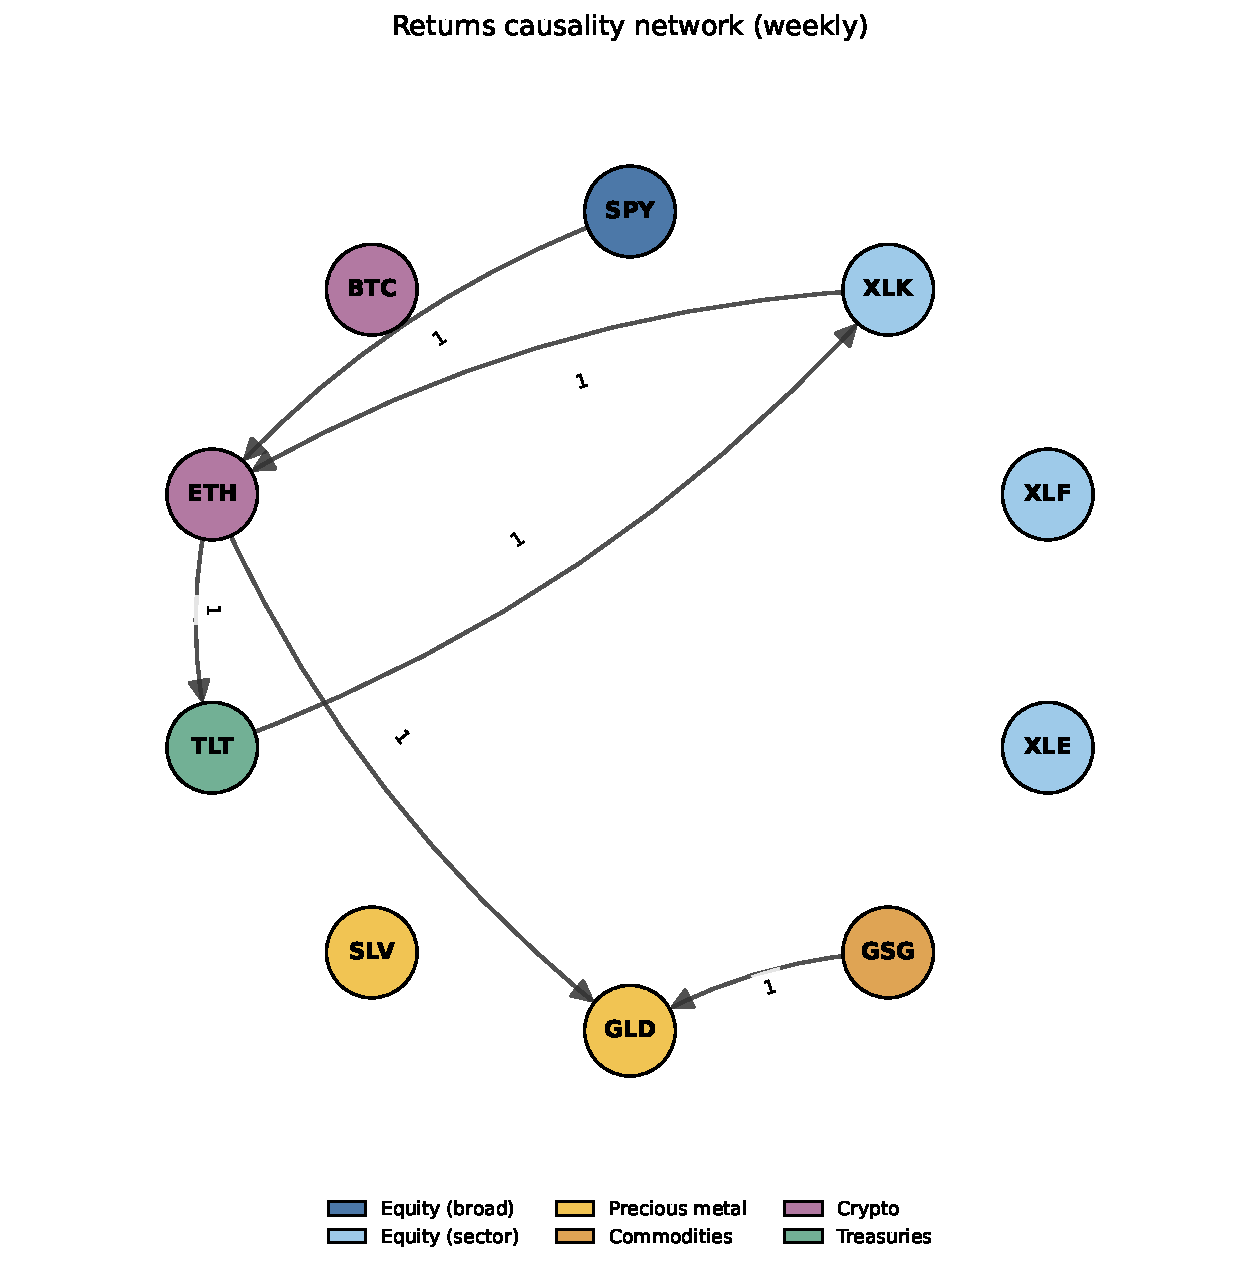
\includegraphics[width=\linewidth]{output/ex1/18_ex1_network_returns_weekly.pdf}
\caption{Weekly.}
\label{fig:net_ret_w}
\end{subfigure}\hfill
\begin{subfigure}[t]{0.49\linewidth}
\centering
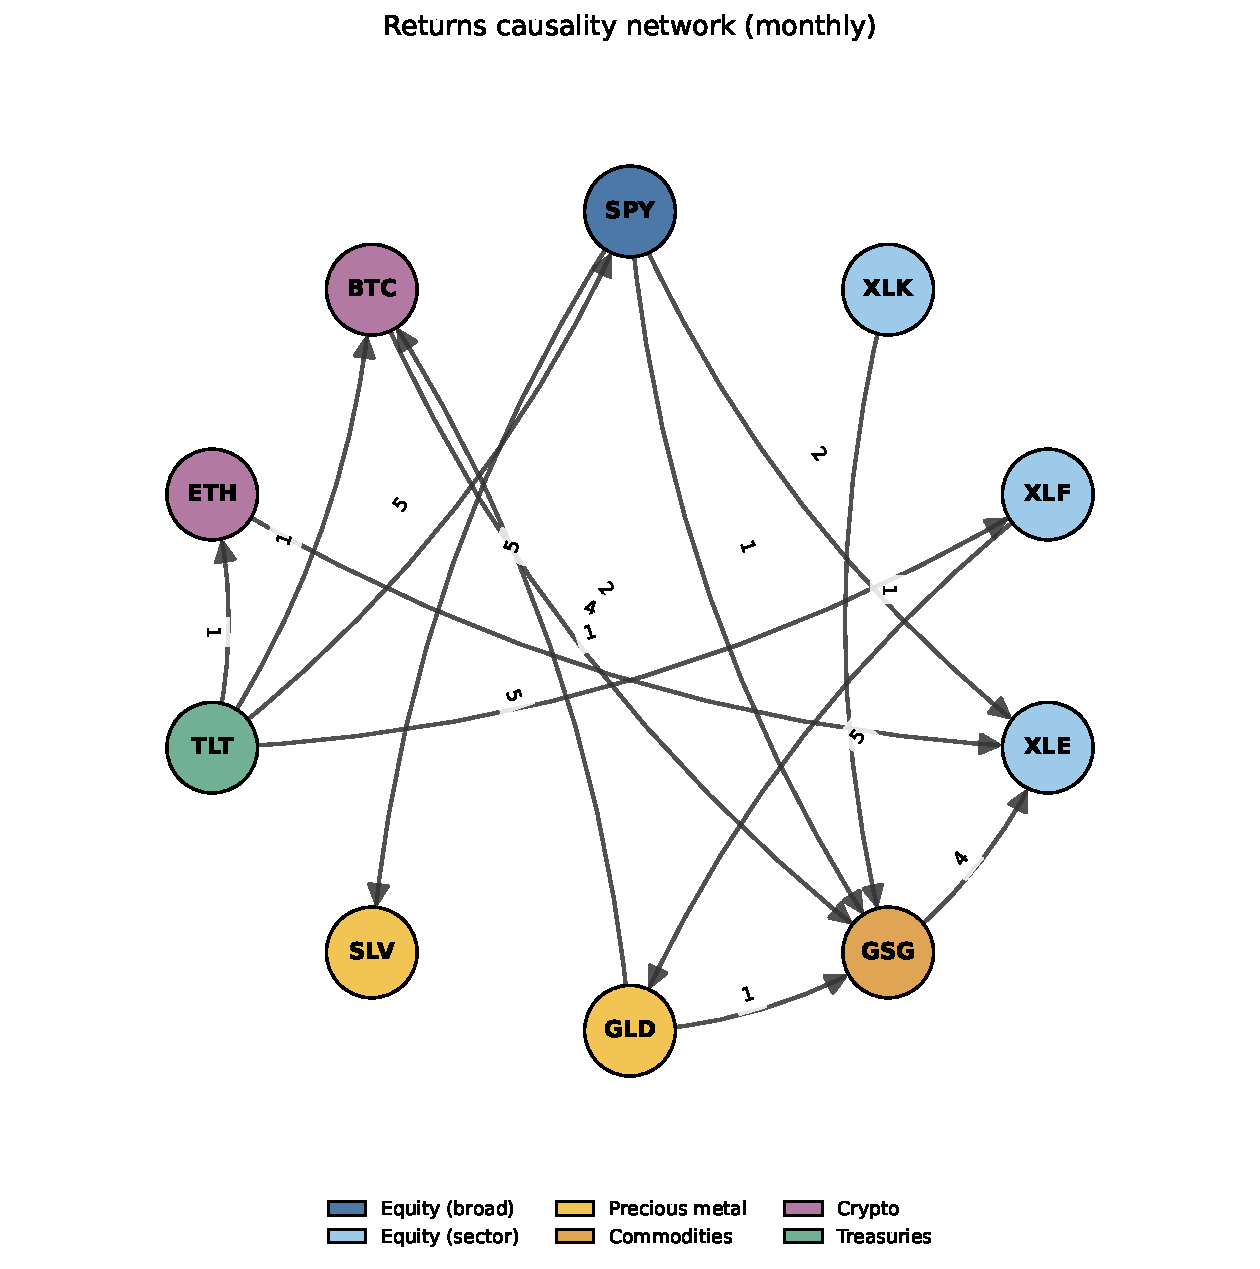
\includegraphics[width=\linewidth]{output/ex1/19_ex1_network_returns_monthly.pdf}
\caption{Monthly.}
\label{fig:net_ret_m}
\end{subfigure}
\caption{Returns-causality networks. Edges run from cause to effect. The integer label is the AIC-optimal VAR lag at which the Granger test rejects at 5\%.}
\label{fig:net_returns}
\end{figure}

The weekly returns network is sparse: \exOneEdgesRW significant directed edges out of ninety ordered pairs, or roughly 7\%. Every selected lag equals one, consistent with broadly efficient secondary markets in which any predictability beyond a single week is quickly arbitraged away. The surviving edges concentrate around ETH. SPY and XLK both Granger-cause weekly Ether returns, and Ether in turn leads the weekly returns of TLT and GLD. We read this as a behavioural channel. In 2024-2025, risk-on/risk-off shifts in equities (and especially in tech, which now drives the index) propagate into crypto with a one-week lag through the marginal retail and institutional investor who rebalances slowly between the two asset classes. The link from ETH to TLT and GLD is best read as a sentiment proxy: weeks of strong crypto performance are often followed by the unwind of safe-haven positions in long Treasuries and gold one week later. The remaining edge GSG~$\rightarrow$~GLD captures the 2024 narrative in which broad commodities (heavily weighted to oil) led precious metals as an early signal of inflation persistence, with gold then catching up.

Moving to monthly sampling the network thickens substantially (\exOneEdgesRM edges), the selected lags spread across the whole admissible range and TLT and SPY emerge as causal hubs. Long Treasuries Granger-cause SPY at lag 5, XLF at lag 1 and both BTC and ETH at lag 1. This mirrors the well-documented role of the long end of the yield curve as the discount-rate channel through which monetary-policy expectations transmit to risky assets. SPY itself Granger-causes XLE (lag 2), SLV (lag 5) and GSG (lag 1), while XLK leads GSG at lag 1. That picture is consistent with a sample that spans the equity-led commodity rebound of mid-2024 and the late-2025 reflation. A caveat is in order. With only \exOneMonthlyReturns monthly observations, AIC frequently selects the boundary lag of 5, a signal that the lag-selection procedure is at the limit of its usable range. We therefore treat the longest-lag edges as borderline. Concretely, a bivariate VAR$(5)$ on a \exOneMonthlyReturns-observation series fits eleven parameters per equation on eighteen post-lag observations. The effective degrees of freedom for each Granger F-test are therefore small, and a non-trivial fraction of the rejected nulls are expected to be sample-specific. Reading the two frequencies jointly recovers a standard lesson. High-frequency returns are very close to a martingale and admit only a handful of one-step predictabilities, whereas monthly horizons make macro-driven persistence detectable at the cost of much larger sampling uncertainty.

The contemporaneous correlation structure helps explain these results. Weekly correlations are \exOneCorrSPYXLKWeekly between SPY and XLK, \exOneCorrGLDSLVWeekly between the two precious metals and \exOneCorrBTCETHWeekly between BTC and ETH. Cross-block correlations sit almost entirely below 0.35 in absolute value. The large within-block correlations explain why most within-block ordered pairs (for instance SPY and XLK) carry no Granger arrow even though the two assets clearly co-move. When two series are nearly contemporaneous, the within-block predictability is absorbed by the contemporaneous correlation and the lagged cross terms add little marginal information.

\probsub{1c}{Volatility Spillover Networks}

Tables~\ref{tab:vol_weekly} and~\ref{tab:vol_monthly} report the directed volatility spillover lag tables and Figure~\ref{fig:net_vol} plots the corresponding networks.

\begin{table}[H]
\centering
\small
\begin{tabular}{lcccccccccc}
\toprule
 & SPY & XLK & XLF & XLE & GLD & SLV & GSG & BTC & ETH & TLT \\
\midrule
SPY & - & 0 & 0 & 0 & 2 & 0 & 2 & 1 & 0 & 2 \\
XLK & 0 & - & 0 & 0 & 2 & 0 & 2 & 0 & 0 & 2 \\
XLF & 1 & 0 & - & 0 & 2 & 0 & 1 & 1 & 0 & 2 \\
XLE & 0 & 0 & 0 & - & 2 & 0 & 1 & 1 & 0 & 2 \\
GLD & 0 & 0 & 0 & 0 & - & 0 & 0 & 2 & 0 & 0 \\
SLV & 0 & 0 & 0 & 0 & 0 & - & 0 & 1 & 0 & 2 \\
GSG & 0 & 0 & 0 & 0 & 0 & 0 & - & 0 & 0 & 2 \\
BTC & 0 & 0 & 0 & 0 & 2 & 0 & 0 & - & 0 & 0 \\
ETH & 0 & 0 & 0 & 0 & 0 & 0 & 0 & 0 & - & 0 \\
TLT & 0 & 0 & 0 & 0 & 0 & 0 & 0 & 0 & 0 & - \\
\bottomrule
\end{tabular}
\caption{Pairwise Granger causality on weekly EWMA volatility. Entries as in the returns tables. \textit{Notes:} The test is applied to EWMA volatility states. A non-zero cell means volatility in the row asset helps forecast volatility in the column asset after the column asset's own volatility history is used.}
\label{tab:vol_weekly}
\end{table}

\begin{table}[H]
\centering
\small
\begin{tabular}{lcccccccccc}
\toprule
 & SPY & XLK & XLF & XLE & GLD & SLV & GSG & BTC & ETH & TLT \\
\midrule
SPY & - & 0 & 0 & 2 & 0 & 0 & 2 & 0 & 0 & 0 \\
XLK & 1 & - & 1 & 0 & 0 & 0 & 5 & 0 & 0 & 0 \\
XLF & 0 & 0 & - & 1 & 0 & 0 & 0 & 0 & 0 & 0 \\
XLE & 0 & 1 & 0 & - & 0 & 0 & 0 & 0 & 4 & 0 \\
GLD & 0 & 5 & 0 & 0 & - & 5 & 0 & 0 & 5 & 0 \\
SLV & 0 & 0 & 0 & 0 & 0 & - & 0 & 0 & 0 & 0 \\
GSG & 0 & 5 & 0 & 0 & 0 & 0 & - & 0 & 4 & 0 \\
BTC & 0 & 0 & 0 & 0 & 1 & 0 & 0 & - & 1 & 0 \\
ETH & 0 & 0 & 0 & 0 & 0 & 0 & 0 & 0 & - & 0 \\
TLT & 0 & 0 & 0 & 2 & 0 & 0 & 2 & 0 & 0 & - \\
\bottomrule
\end{tabular}
\caption{Pairwise Granger causality on monthly EWMA volatility. Entries as in the returns tables. \textit{Notes:} Monthly volatility mixes EWMA memory with calendar aggregation. Long delays may describe slow risk regimes. They may also reflect limited monthly data.}
\label{tab:vol_monthly}
\end{table}


\begin{figure}[H]
\centering
\begin{subfigure}[t]{0.49\linewidth}
\centering
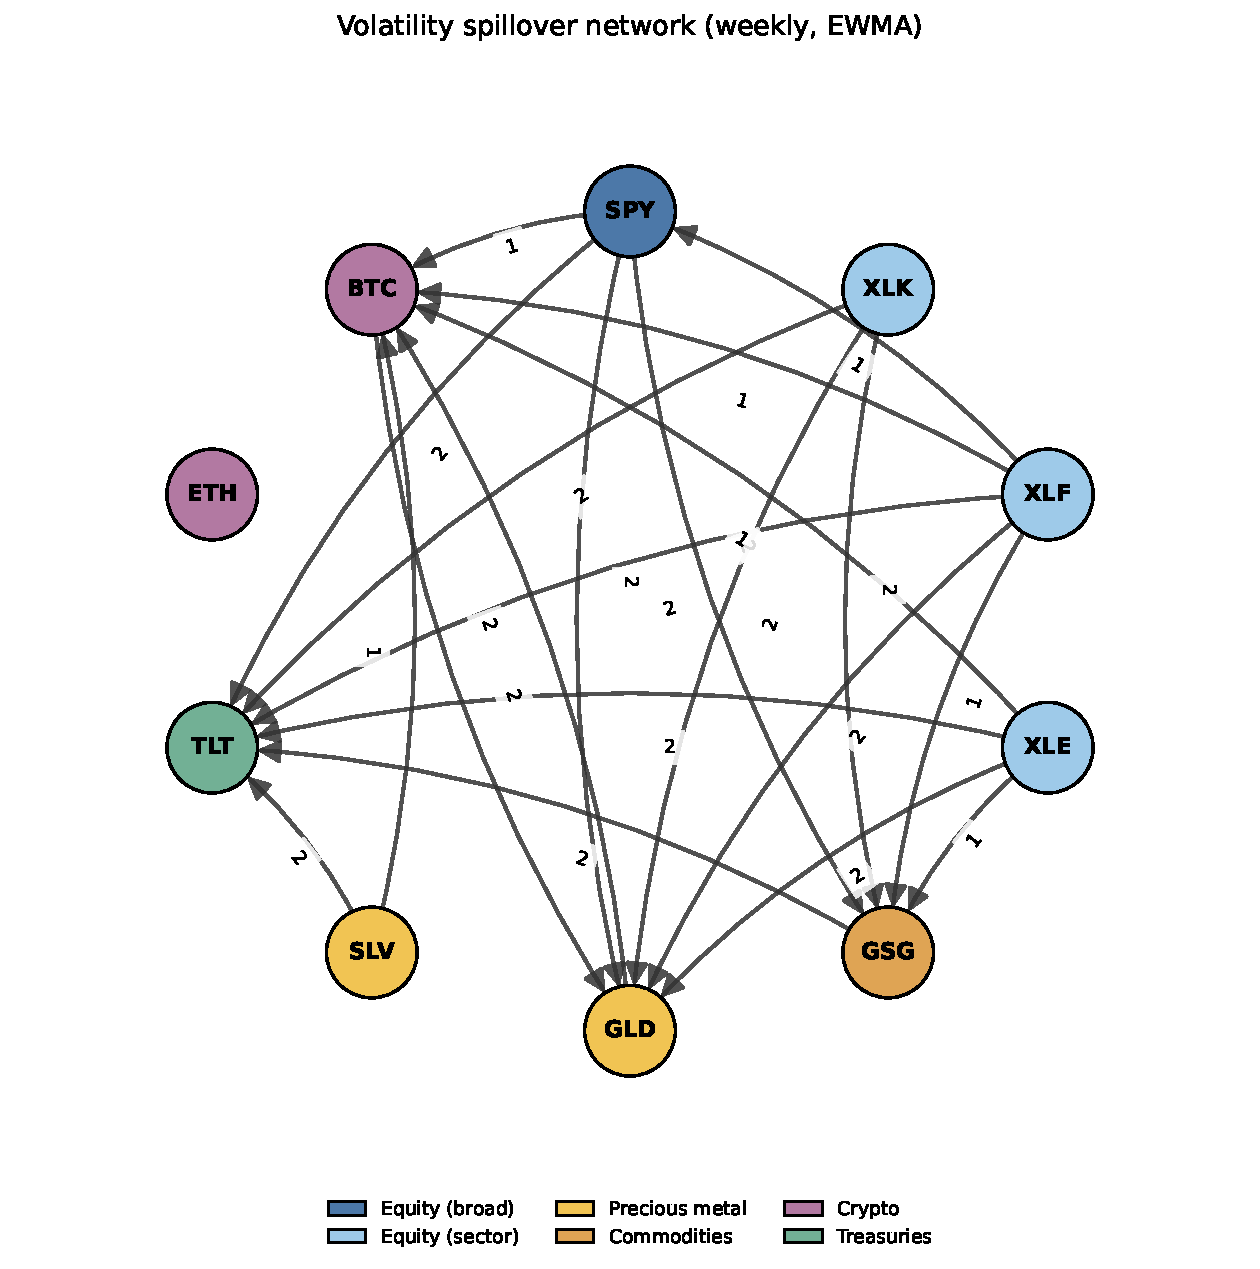
\includegraphics[width=\linewidth]{output/ex1/20_ex1_network_vol_weekly.pdf}
\caption{Weekly.}
\label{fig:net_vol_w}
\end{subfigure}\hfill
\begin{subfigure}[t]{0.49\linewidth}
\centering
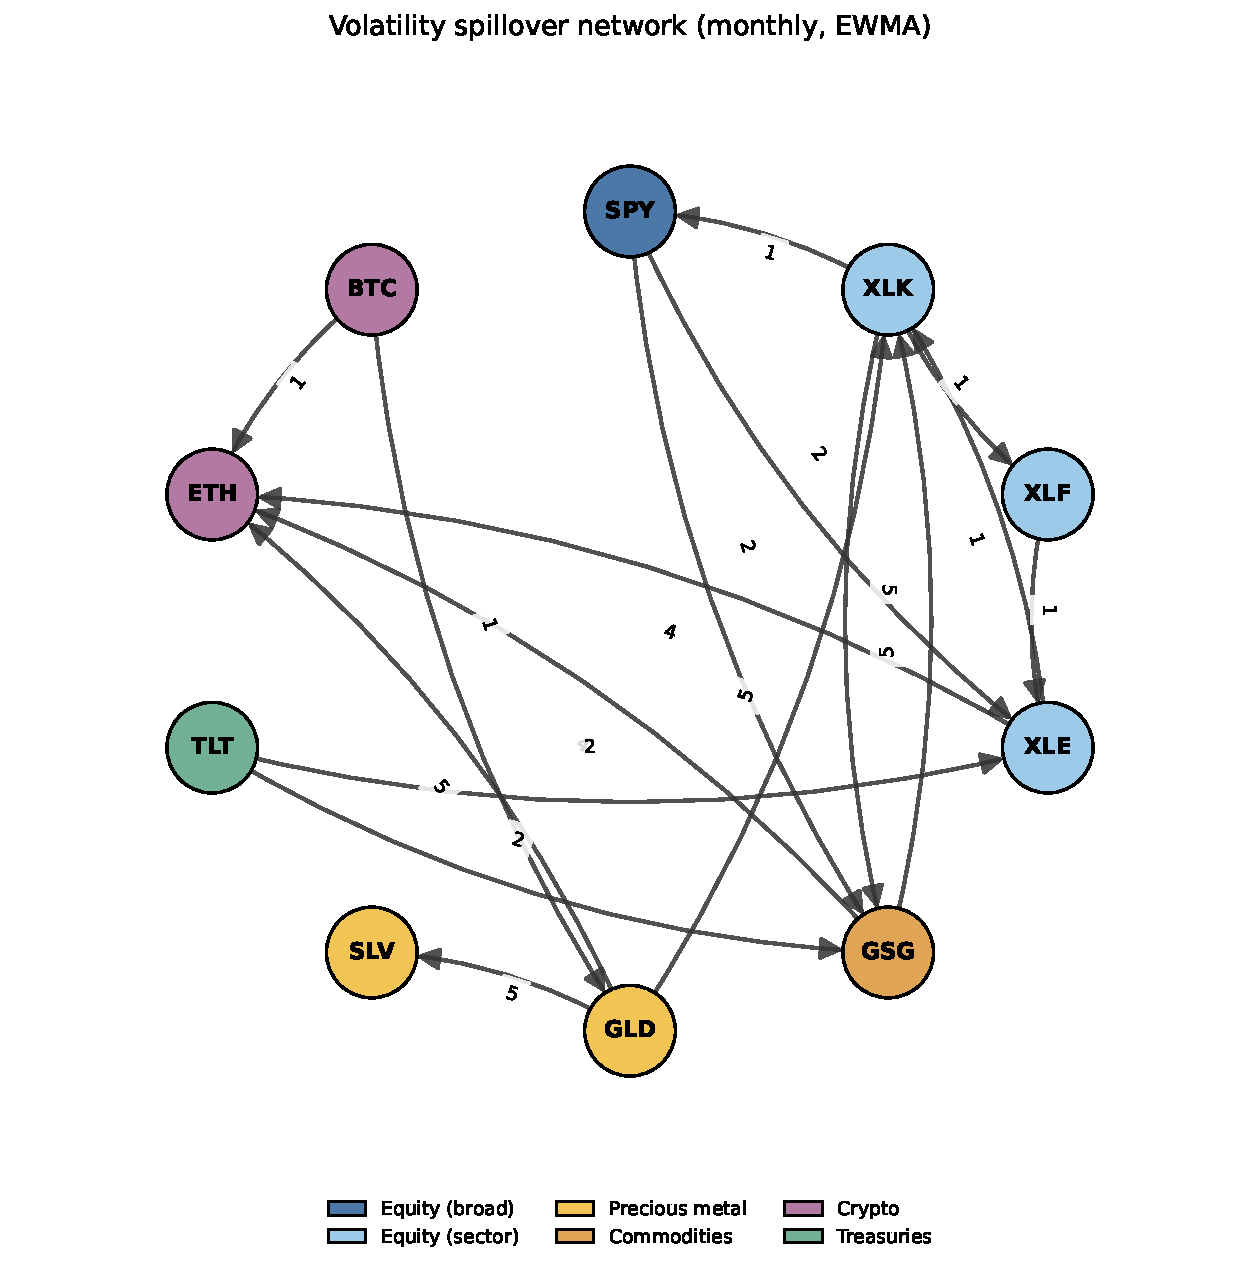
\includegraphics[width=\linewidth]{output/ex1/21_ex1_network_vol_monthly.pdf}
\caption{Monthly.}
\label{fig:net_vol_m}
\end{subfigure}
\caption{EWMA volatility spillover networks (RiskMetrics, $\lambda{=}0.94$). Edges run from cause to effect. The integer label is the AIC-optimal VAR lag at which the Granger test rejects at 5\%.}
\label{fig:net_vol}
\end{figure}

Volatility produces several times more significant edges than returns at the same frequency: \exOneEdgesVW weekly and \exOneEdgesVM monthly volatility edges against \exOneEdgesRW weekly and \exOneEdgesRM monthly return edges. Realised volatility is highly persistent. EWMA carries past shocks forward recursively with a per-period half-life of $\log(0.5)/\log(\lambda) \approx \exOneEwmaHalfLife$ periods at $\lambda{=}\exOneEwmaLambda$. Once two assets share even a moderate exposure to the same volatility regime, lagged cross terms become statistically informative even when the contemporaneous return correlation is modest. The channels identified here therefore describe the propagation of the second-order risk regime.

The weekly spillover network is dominated by equity-block sources. SPY, XLK, XLF and XLE each emit several directed arrows (mostly at lag 2), with TLT, GLD and GSG appearing repeatedly as receivers. This is the familiar shape of a ``fear'' map: when the equity volatility regime tightens, the volatility of safe-haven assets and broad commodities adjusts one or two weeks later. The lag reflects investors rebalancing hedges and macro-trend strategies digesting the new variance level. A two-week delay is consistent with the typical rebalancing window of monthly-mandate funds and with the time it takes for option-implied vol to pass through to realised cross-asset vol. ETH is essentially isolated in the weekly volatility map, while BTC receives edges from XLF (lag 1), SPY (lag 1) and XLE (lag 1). The 2024-2025 window contains the spot-Bitcoin-ETF approval of January 2024 and the post-election crypto rally, both of which plausibly tightened the link between Bitcoin volatility and the equity regime, while Ether decoupled on idiosyncratic supply-side news.

The monthly picture is qualitatively similar but the channels reorder. The main causal cluster sits around the precious-metals-and-commodities block: GLD~$\rightarrow$~XLK (lag 5), GLD~$\rightarrow$~SLV (lag 5), GLD~$\rightarrow$~ETH (lag 5), GSG~$\rightarrow$~ETH (lag 4) and GSG~$\rightarrow$~XLK (lag 5). XLK is fed at the long horizon by XLE (lag 1), GLD (lag 5) and GSG (lag 5), while emitting causally to SPY (lag 1), XLF (lag 1) and GSG (lag 5). It sits at the centre of the equity-block and equity-to-commodities transmission. These long-lag arrows largely reflect the \exOneMonthlyReturns-observation small-sample regime in which AIC frequently selects the boundary lag of 5. We read them as suggestive of a slow inflation-and-real-rates channel through which commodity volatility shocks gradually feed equity-sector volatility, with the usual caveat that the sample is short.

Contemporaneous correlations on the volatility side make the small-sample issue explicit. At monthly frequency the absolute correlation between SPY-vol and ETH-vol reaches \exOneCorrSPYETHVolMonthly, between BTC-vol and SPY-vol \exOneCorrSPYBTCVolMonthly and between GLD-vol and SPY-vol $\exOneCorrSPYGLDVolMonthly$ (i.e.\ 0.91 in absolute value, sign negative). With \exOneMonthlyReturns observations and bilateral correlations this large, the bivariate VARs are estimated on data with very little independent information. Many of the long-lag edges are likely contaminated by the weekly-EWMA propagation of a single common volatility shock, notably the August 2024 yen-carry unwind and the spring 2025 tariff scare. Weekly correlations sit in the 0.5 to 0.9 range, where the network is more credible.

In summary, the returns network is broadly consistent with weak-form efficient markets at high frequency, with only modest monthly predictability driven by the rates channel (TLT~$\rightarrow$~SPY, TLT~$\rightarrow$~financials and TLT~$\rightarrow$~crypto). The volatility network is far denser. The equity block (SPY, XLK, XLF and XLE) is the main source of weekly fear, with TLT, GLD and GSG as receivers. At the monthly horizon the precious-metals-and-energy block takes on a more central role. The asymmetry between return sparsity and volatility density is the data-science finding of this exercise: prices are hard to predict, while the second-moment regime propagates broadly across assets.

% =============================================================================
% Exercise 2
% =============================================================================
\probsection{2}{Forecasting the S\&P 500 with Fundamental Indicators}

We forecast the monthly S\&P 500 series over 1927-2021 with our team-assigned Goyal-Welch indicators (dp, svar and bm) plus lags of these indicators and lags of the target. A multilayer perceptron, an LSTM and a Gaussian-process regression are compared across three target specifications (return, price and direction), and we ask which target works best. We also perform feature selection and a sensitivity analysis on the exogenous variables. The pipeline lives in the notebook \code{scripts/exercise\_02.ipynb}, which we ran on a Colab GPU runtime. The artefacts we discuss below live in \code{output/ex2/}.

\probsub{2a}{Feature Selection and Target Design}

We load the Goyal-Welch monthly file, restrict to 1927-01 to 2021-12 and construct the three target series,
\begin{equation}
r_{t+1} \;=\; \log P_{t+1} - \log P_t,\qquad
p_{t+1} \;=\; \log P_{t+1},\qquad
d_{t+1} \;=\; \mathbf{1}\{r_{t+1} > 0\},
\label{eq:targets}
\end{equation}
giving 1140 monthly observations after the NA-drop. The three targets in~\eqref{eq:targets} live at time $t{+}1$ and are predicted from features observed at $t$ and earlier, so the design avoids any forward-looking contamination. Features are the lags 1, 2 and 3 of the natural target series (log return for return and direction. Log price for price) plus the lags 1, 2 and 3 of dp, svar and bm: 12 candidate features in total. We split chronologically into 60\% training (\exTwoNTrain obs), 15\% validation (\exTwoNVal obs) and 25\% test (\exTwoNTest obs). The validation block selects hyperparameters, after which the final model is refit on the train$+$validation block before scoring on the held-out test set. The L1 feature-selection step and the inner cross-validation it relies on use a \code{TimeSeriesSplit} so that no fold ever validates on data preceding the data it was trained on. Feature scaling and the L1 selection step (\code{LassoCV} for return and price. $\ell_1$-penalised \code{LogisticRegressionCV} for direction) are fitted on the training set only and applied to validation and test. We compare a multilayer perceptron over an 8-cell grid (hidden sizes $(64,)$, $(128,)$, $(64,64)$ and $(128,64)$, each with ReLU and tanh), a Gaussian-process regressor over four kernels (RBF, Matern with $\nu=2.5$, RationalQuadratic and a custom non-stationary additive RBF$+$Linear$+$WhiteNoise) with two restarts of the kernel-hyperparameter optimiser and an LSTM over a 4-cell grid varying width (32 and 64), depth (1 and 2 layers) and timestep window (6 and 12) with early stopping on a 10\% internal validation slice. Each model picks its best configuration on the validation NRMSE (accuracy for direction), then refits on train$+$validation and is scored on the held-out test set. We report the normalised RMSE,
\begin{equation}
\mathrm{NRMSE}(\hat y) \;=\; \sqrt{\dfrac{\mathrm{MSE}(\hat y, y)}{\overline{\sum_t (y_t - \bar y)^2}}},
\qquad \mathrm{pcorrect} \;=\; 100 (1 - \mathrm{NRMSE}),
\label{eq:nrmse}
\end{equation}
together with raw RMSE for the regression targets and accuracy and the Matthews correlation coefficient (MCC) for the direction target. The pcorrect form in~\eqref{eq:nrmse} is the lab convention, not the sklearn definition. The naive benchmarks are the in-sample mean for the regression targets and the in-sample majority class for direction.

The Lasso step itself yields a first observation. On the return target the surviving features are \exTwoFeaturesReturn: lags of dp and svar are shrunk to zero, and only the third lag of the target itself survives alongside two book-to-market lags. The price target retains \exTwoFeaturesPrice, where the lagged log price dominates as expected and a small handful of indicator lags is kept. Direction is the most permissive case: the L1 logistic with \code{TimeSeriesSplit} inner CV keeps eleven of the twelve candidate lags (only dp\_lag2 is dropped), so the classifier sees almost the full feature set. At the monthly horizon the autoregressive component (lagged log returns and lagged log price) carries most of the information the L1 selector keeps. Among the assigned indicators, book-to-market is the most consistently retained.

\probsub{2b}{Return Forecasts}

Table~\ref{tab:ex2_return} reports the test-set performance of the three models on the return target. Figure~\ref{fig:ex2_return} plots predictions against realised returns.

\begin{table}[H]
\centering
\small
\begin{tabular}{lllcccc}
\toprule
Model & Best configuration & RMSE & NRMSE & pcorrect \\
\midrule
NN            & 2 layers, $(128,64)$, ReLU       & \exTwoReturnNNRMSE          & \exTwoReturnNNNRMSE          & \exTwoReturnNNPcorrect \\
GP            & RBF + WhiteNoise                  & \exTwoReturnGPRMSE          & \exTwoReturnGPNRMSE          & \exTwoReturnGPPcorrect \\
LSTM          & 1 layer, 64 units, $T{=}6$        & \exTwoReturnLSTMRMSE        & \exTwoReturnLSTMNRMSE        & \exTwoReturnLSTMPcorrect \\
BaselineMean  & predict in-sample mean            & \exTwoReturnBaselineMeanRMSE & \exTwoReturnBaselineMeanNRMSE & \exTwoReturnBaselineMeanPcorrect \\
\bottomrule
\end{tabular}
\caption{Test-set forecast performance for the return target ($n=285$). The BaselineMean predicts the in-sample training mean of $\log r$. Pcorrect $= 100(1-\mathrm{NRMSE})$.}
\label{tab:ex2_return}
\end{table}

\begin{figure}[H]
\centering
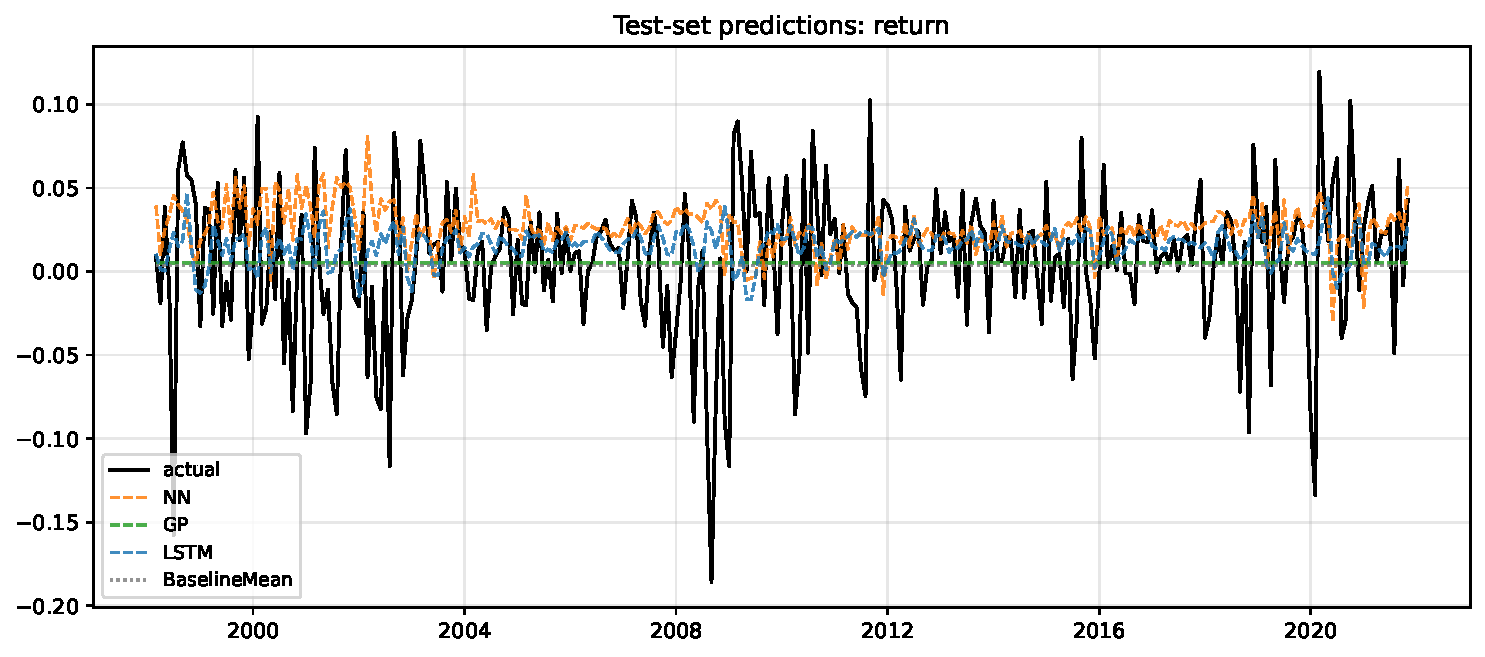
\includegraphics[width=0.95\linewidth]{output/ex2/07_ex2_fig_return.pdf}
\caption{Test-set predictions of next-month log return. The actual series (black) is volatile in the $\pm 10\%$ range. Every model flatlines near zero and is statistically indistinguishable from the in-sample mean baseline.}
\label{fig:ex2_return}
\end{figure}

No model beats the in-sample mean baseline at any meaningful level of significance. The GP essentially ties the baseline (NRMSE \exTwoReturnGPNRMSE against \exTwoReturnBaselineMeanNRMSE), the LSTM is about 0.4 percentage points of NRMSE worse and the NN is about 1.1 percentage points worse. The deeper $(128,64)$ ReLU architecture chosen by the validation grid produces a noisier fit than the simpler GP. This is the textbook outcome for a near-martingale series. On monthly data the conditional mean of log returns, given any subset of past observables and Goyal-Welch indicators, is statistically indistinguishable from the unconditional mean. The optimal MSE-minimising forecast is therefore the unconditional mean, which is what the naive baseline computes. The figure makes the same point visually: actual returns oscillate in the $\pm 10\%$ range while every model sits in a narrow band near zero, capturing essentially none of the dispersion. We read this as direct empirical support for the weak form of the efficient-markets hypothesis on the post-1998 test window.

\probsub{2c}{Log-Price Forecasts}

The price-target results are collected in Table~\ref{tab:ex2_price}, with Figure~\ref{fig:ex2_price} plotting predictions against realised log prices.

\begin{table}[H]
\centering
\small
\begin{tabular}{lllcccc}
\toprule
Model & Best configuration & RMSE & NRMSE & pcorrect \\
\midrule
NN            & 1 layer, 64 units, ReLU            & \exTwoPriceNNRMSE          & \exTwoPriceNNNRMSE          & \exTwoPriceNNPcorrect \\
GP            & custom RBF + Linear + WhiteNoise   & \exTwoPriceGPRMSE          & \exTwoPriceGPNRMSE          & \exTwoPriceGPPcorrect \\
LSTM          & 1 layer, 64 units, $T{=}6$         & \exTwoPriceLSTMRMSE        & \exTwoPriceLSTMNRMSE        & \exTwoPriceLSTMPcorrect \\
BaselineMean  & predict in-sample mean             & \exTwoPriceBaselineMeanRMSE & \exTwoPriceBaselineMeanNRMSE & \exTwoPriceBaselineMeanPcorrect \\
\bottomrule
\end{tabular}
\caption{Test-set forecast performance for the price target, $\log P_{t+1}$ ($n=285$).}
\label{tab:ex2_price}
\end{table}

\begin{figure}[H]
\centering
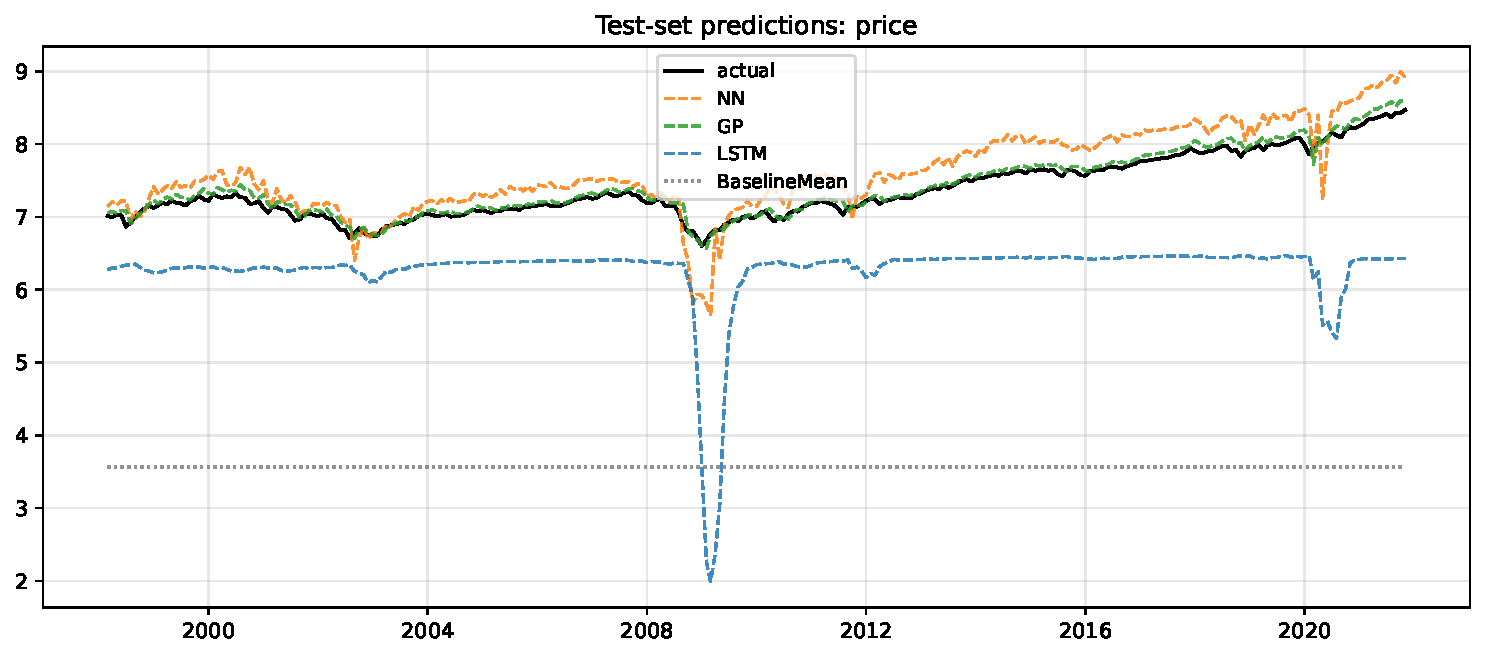
\includegraphics[width=0.95\linewidth]{output/ex2/09_ex2_fig_price.pdf}
\caption{Test-set predictions of next-month log price. NN and GP track the actual series tightly with a small upward bias. The LSTM produces a flat trajectory with a misplaced spike at the 2008 crisis. The in-sample-mean baseline is constant at the training-set average of $\log P$ and is therefore visually pinned at $\approx 3.6$, far below the test sample.}
\label{fig:ex2_price}
\end{figure}

The price-target picture inverts. Every model beats the mean baseline by a factor of 3 to 50 in NRMSE. The GP with the custom non-stationary additive kernel (RBF $+$ Linear $+$ WhiteNoise) is the best of the four (NRMSE \exTwoPriceGPNRMSE against \exTwoPriceNNNRMSE for the NN and \exTwoPriceLSTMNRMSE for the LSTM). The dominant feature in this regression is log\_price\_lag1: predicting tomorrow's log price as approximately today's log price plus a small drift recovers most of the variance, because the price series is integrated of order one. The custom kernel captures this directly, with the Linear (DotProduct) component handling the long-run drift and the RBF component capturing local curvature around the trend. The LSTM struggles because its 6-step input window does not naturally encode the long-run level. Seeing only the last six normalised observations, it produces a flat extrapolation that mis-times the 2008 crash with a downward spike (visible in Figure~\ref{fig:ex2_price}). The apparent \exTwoPriceGPPcorrect\% pcorrect for the GP is largely a tautology. Forecasting log price one step ahead is essentially a random-walk-with-drift problem, and any model that sees the lagged log price inherits nearly all of the explanatory power from the autoregressive root. The substantive question is whether any model extracts additional predictive information from the Goyal-Welch indicators beyond what the lagged price already supplies. The answer is: a little.

\probsub{2d}{Direction Forecasts}

For the direction target, Table~\ref{tab:ex2_direction} gives the test-set scores and Figure~\ref{fig:ex2_direction} plots predictions against the realised directions.

\begin{table}[H]
\centering
\small
\begin{tabular}{llcc}
\toprule
Model & Best configuration & accuracy & MCC \\
\midrule
NN                 & 1 layer, 128 units, tanh        & \exTwoDirectionNNAccuracy                & $\exTwoDirectionNNMCC$ \\
GP                 & RatQuad + WhiteNoise            & \exTwoDirectionGPAccuracy                & $\phantom{-}\exTwoDirectionGPMCC$ \\
LSTM               & 2 layers, 32 units, $T{=}6$     & \exTwoDirectionLSTMAccuracy              & $\exTwoDirectionLSTMMCC$ \\
BaselineMajority   & predict the in-sample majority  & \exTwoDirectionBaselineMajorityAccuracy  & $\phantom{-}\exTwoDirectionBaselineMajorityMCC$ \\
\bottomrule
\end{tabular}
\caption{Test-set forecast performance for the direction target ($n=285$, test period 1998-03 to 2021-11). The 0.6246 accuracy of the BaselineMajority equals the unconditional up-rate over the test set. The GP also degenerates to the majority class while the NN and the LSTM produce non-trivial predictions with negative MCC. The direction column is constructed inside the design step from $\mathbf{1}\{r_{t+1} > 0\}$ on the restricted panel, so the $t{+}1$ alignment stays inside the assignment's 1927-2021 window.}
\label{tab:ex2_direction}
\end{table}

\begin{figure}[H]
\centering
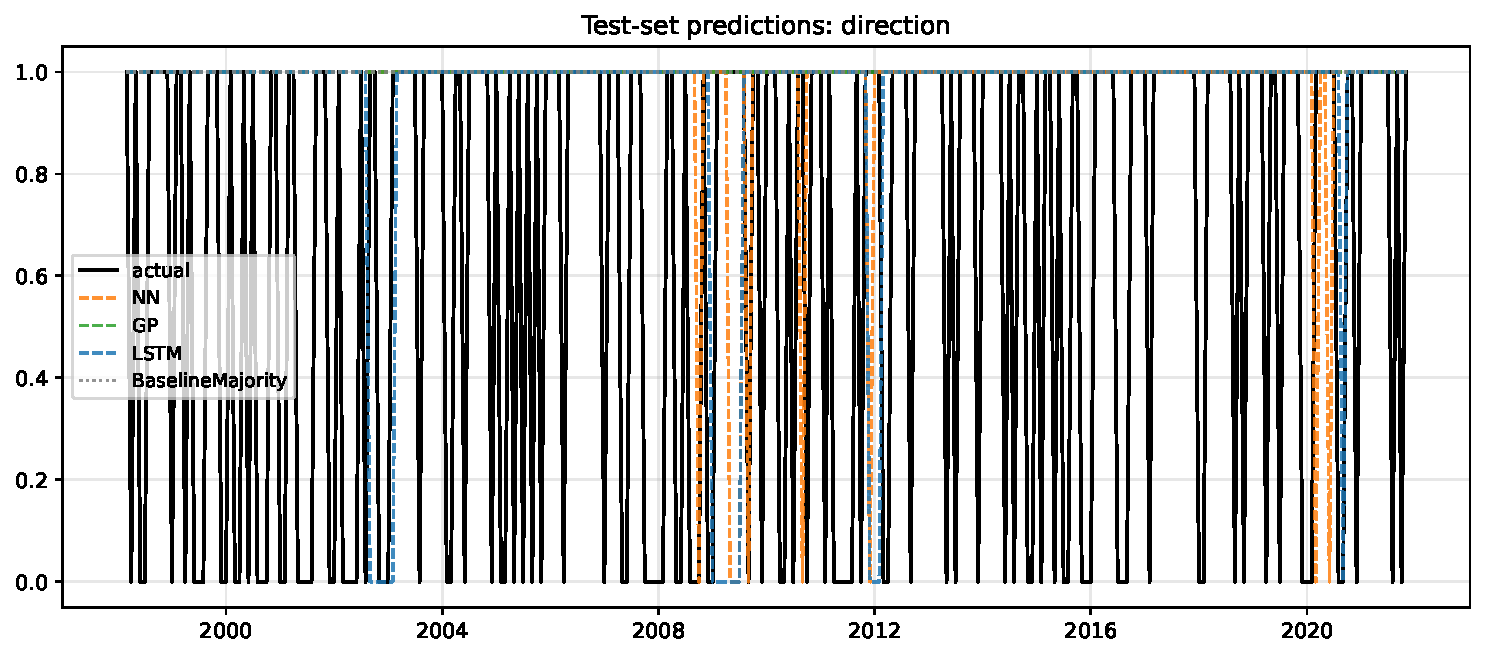
\includegraphics[width=0.95\linewidth]{output/ex2/11_ex2_fig_direction.pdf}
\caption{Test-set predictions of next-month direction. The GP and BaselineMajority predict $\hat d \equiv 1$. The NN and LSTM toggle to 0 on a small fraction of the test months (visible as occasional downward spikes in the orange and blue dashed lines) and the resulting class assignments produce a slightly negative Matthews correlation.}
\label{fig:ex2_direction}
\end{figure}

The direction target tells a more nuanced story than the return target. The GP and the BaselineMajority both degenerate to the constant prediction $\hat d_{t+1} \equiv 1$ and therefore land at the unconditional up-rate accuracy of \exTwoDirectionBaselineMajorityAccuracy with Matthews correlation exactly zero. The NN and the LSTM flip a non-zero number of class assignments: the NN sits at \exTwoDirectionNNAccuracy accuracy with MCC \exTwoDirectionNNMCC, and the LSTM at \exTwoDirectionLSTMAccuracy with MCC \exTwoDirectionLSTMMCC. Both negative MCCs say that the models are slightly worse than random on this test set, even though they are strictly less degenerate than the majority-class baseline. The L1 logistic with \code{TimeSeriesSplit} inner CV kept almost the full feature pool for the direction problem (eleven of the twelve candidates), so the NN and LSTM picked up sample-specific patterns that fail to generalise. The MCC is the diagnostic that distinguishes a model that genuinely uses the features (non-zero MCC) from a model that defaults to the majority class (zero MCC).

\probsub{2e}{Sensitivity Analysis}

For the sensitivity analysis we drop, in turn, all lags of dp, of svar and of bm from the candidate feature pool and re-run the full feature-selection-and-fit pipeline. Table~\ref{tab:ex2_sensitivity} reports the test-set NRMSE for the regression targets and the test-set accuracy for the direction target. Differences from the main run isolate the marginal contribution of each indicator.

\begin{table}[H]
\centering
\small
\begin{tabular}{llccc}
\toprule
Target & Dropped & NN (NRMSE) & GP (NRMSE) & LSTM (NRMSE) \\
\midrule
return & (none) & \exTwoReturnNNNRMSE                 & \exTwoReturnGPNRMSE                 & \exTwoReturnLSTMNRMSE \\
return & dp     & \exTwoSensReturnNNDropDpNRMSE       & \exTwoSensReturnGPDropDpNRMSE       & \exTwoSensReturnLSTMDropDpNRMSE \\
return & svar   & \exTwoSensReturnNNDropSvarNRMSE     & \exTwoSensReturnGPDropSvarNRMSE     & \exTwoSensReturnLSTMDropSvarNRMSE \\
return & bm     & \exTwoSensReturnNNDropBmNRMSE       & \exTwoSensReturnGPDropBmNRMSE       & \exTwoSensReturnLSTMDropBmNRMSE \\
\midrule
price  & (none) & \exTwoPriceNNNRMSE                  & \exTwoPriceGPNRMSE                  & \exTwoPriceLSTMNRMSE \\
price  & dp     & \exTwoSensPriceNNDropDpNRMSE        & \exTwoSensPriceGPDropDpNRMSE        & \exTwoSensPriceLSTMDropDpNRMSE \\
price  & svar   & \exTwoSensPriceNNDropSvarNRMSE      & \exTwoSensPriceGPDropSvarNRMSE      & \exTwoSensPriceLSTMDropSvarNRMSE \\
price  & bm     & \exTwoSensPriceNNDropBmNRMSE        & \exTwoSensPriceGPDropBmNRMSE        & \exTwoSensPriceLSTMDropBmNRMSE \\
\midrule
\multicolumn{5}{l}{(direction is reported as accuracy)} \\
direction & (none) & \exTwoDirectionNNAccuracy           & \exTwoDirectionGPAccuracy           & \exTwoDirectionLSTMAccuracy \\
direction & dp     & \exTwoSensDirectionNNDropDpAccuracy & \exTwoSensDirectionGPDropDpAccuracy & \exTwoSensDirectionLSTMDropDpAccuracy \\
direction & svar   & \exTwoSensDirectionNNDropSvarAccuracy & \exTwoSensDirectionGPDropSvarAccuracy & \exTwoSensDirectionLSTMDropSvarAccuracy \\
direction & bm     & \exTwoSensDirectionNNDropBmAccuracy & \exTwoSensDirectionGPDropBmAccuracy & \exTwoSensDirectionLSTMDropBmAccuracy \\
\bottomrule
\end{tabular}
\caption{Sensitivity analysis. Each row is the test-set performance when all lags of the indicated variable are removed from the candidate feature pool before Lasso selection. NRMSE is reported for return and price, accuracy for direction. The GP keeps the same single best kernel across most ablations because its hyperparameters are re-optimised on the smaller feature subset.}
\label{tab:ex2_sensitivity}
\end{table}

The structure of the table mirrors the Lasso finding with several reversals. On the return target the NN improves when dp or svar is dropped (NRMSE falls from \exTwoReturnNNNRMSE in the main run to \exTwoSensReturnNNDropDpNRMSE). The L1 selector picks a slightly different feature subset (and a different best NN architecture) once the candidate pool is restricted, and the smaller subset generalises better. The GP is invariant across all return ablations because its preferred RBF $+$ WhiteNoise solution absorbs uninformative features into the noise term. The price-target GP shows the same pattern: dropping svar or bm improves the fit (NRMSE \exTwoPriceGPNRMSE in the main run, \exTwoSensPriceGPDropSvarNRMSE after dropping svar and \exTwoSensPriceGPDropBmNRMSE after dropping bm). We read this as a mild form of feature-induced overfitting on noisy regressors. The NN improves further when dp is dropped (NRMSE \exTwoSensPriceNNDropDpNRMSE, the best of any (model, ablation) combination on the price target). It then degrades when svar or bm is dropped, indicating that dp is the indicator the NN was misusing. On the direction side, dropping any of the three indicators removes the negative-MCC pathology of the NN and LSTM. With dp dropped, all three models match the majority-class baseline at \exTwoSensDirectionNNDropDpAccuracy accuracy and zero MCC. With svar dropped, the LSTM joins the majority class while the NN still slightly underperforms. With bm dropped, the NN, GP and LSTM all produce small but positive MCCs (\exTwoSensDirectionNNDropBmMCC, \exTwoSensDirectionGPDropBmMCC and \exTwoSensDirectionLSTMDropBmMCC respectively). On this test sample the assigned indicators introduce more noise than signal for direction prediction: removing them either eliminates the spurious patterns or, in the bm-dropped case, leaves a small genuine residual signal in the autoregressive lags.

\probsub{2f}{Target Comparison}

The headline NRMSE numbers and the answer to ``for which target does the model work best?'' are in tension. By NRMSE alone, the price target wins by a wide margin: every model beats the mean baseline by an order of magnitude or more and the GP reaches \exTwoPriceGPPcorrect\% pcorrect. That performance is driven almost entirely by the lagged log-price feature acting as an autoregressive root in a near random-walk. It contributes little evidence about whether the Goyal-Welch indicators help us forecast equity dynamics. The honest comparison is between the return and direction targets, and there the lesson is the same: on this 95-year monthly sample no model beats the unconditional mean for log returns, and no model produces a directional classifier with a positive MCC on the full feature set. We therefore read ``works best'' in two senses. The price target works best in the trivial sense that any model exploiting the autoregressive root will score well. The return target is the most direct forecasting problem, and there the GP with an RBF kernel ties the constant-mean predictor for first place. The direction outcome rests on the sensitivity result: the (NN, GP, LSTM) trio only produces positive MCCs once book-to-market is removed from the candidate features, indicating that on this test sample the assigned indicators introduce more noise than signal for the binary classification problem.

% =============================================================================
% Exercise 3
% =============================================================================
\probsection{3}{ARMA-GARCH Benchmarks}

We compare the Exercise 2 ML models against a classical ARMA(p,q) $+$ GARCH(1,1) baseline together with a normalising transformation of variables. Two variants of the baseline are fit on the same data with the same chronological 60/15/25 split as Exercise 2, so the test sets coincide exactly. The variants are a plain ARMA-GARCH on the raw log-return series and a Yeo-Johnson-normalised ARMA-GARCH whose predictions are inverse-transformed back to the original return scale before scoring. The pipeline is in \code{scripts/exercise\_03.py}. The artefacts live in \code{output/ex3/}.

\probsub{3a}{Model Orders and Volatility Persistence}

We work with the same monthly log-return series as Exercise 2 and fit both ARMA-GARCH variants on the combined train$+$validation block (852 observations, 1927-03 to 1998-02), then score one-step-ahead forecasts on the \exTwoNTest-observation test block (1998-03 to 2021-11). The ARMA order is selected by AIC over $p, q \in \{0, \dots, 5\}$ via \code{pmdarima.auto\_arima} (stepwise search. No differencing since returns are already stationary. No seasonal component for monthly equity returns). After the ARMA fit we layer a GARCH(1,1) on the residuals using the \code{arch} library,
\begin{equation}
r_t \;=\; \mu_t \;+\; a_t,\qquad
\mu_t \;=\; \phi_1 r_{t-1} + \dots + \phi_p r_{t-p} + \theta_1 a_{t-1} + \dots + \theta_q a_{t-q},
\label{eq:arma_mean}
\end{equation}
\begin{equation}
a_t \;=\; \sigma_t \varepsilon_t,\qquad
\sigma_t^2 \;=\; \omega + \alpha_1 a_{t-1}^2 + \beta_1 \sigma_{t-1}^2,\qquad \varepsilon_t \sim \mathcal{N}(0, 1).
\label{eq:garch}
\end{equation}
The conditional-mean term $\mu_t$ in~\eqref{eq:arma_mean} and the conditional-variance recursion in~\eqref{eq:garch} are estimated jointly by quasi-maximum likelihood.
A short remark on what ``normalising'' means here. The log-return transform $r_t = \log P_t - \log P_{t-1}$ is itself a normalising step: it converts a non-Gaussian, integrated price level into a stationary, near-bell-shaped series, which is exactly why ARMA-GARCH is fit to log returns rather than to prices in the first place. The Yeo-Johnson variant is therefore a \emph{second} distribution-matching transformation layered on top of the log-return scale, intended to pull the marginal closer to Gaussian where the residual skewness and kurtosis would otherwise hurt the maximum-likelihood ARMA estimator. For the Yeo-Johnson variant we fit the transformer on the same train$+$validation fitting block used for the ARMA estimator. The test set is never touched. We then apply ARMA-GARCH to the transformed series and inverse-transform the predicted returns back to the original scale. Yeo-Johnson is the natural choice for real-valued data that can include negatives, since it accepts negative inputs as is, while Box-Cox needs strictly positive inputs and the logit transformation needs bounded inputs in $(0,1)$.

One-step-ahead test forecasts are produced by extending the fitted ARMA model with the test endogenous data via \code{ARIMA.apply(refit=False)} and reading the in-sample fitted values for the test block. This is the standard ``static parameters, expanding history'' procedure, which gives genuine one-step-ahead forecasts conditional on the realised path with parameters held fixed throughout the test period. Each forecast at time $t+1$ uses only data observed at or before time $t$, so there is no multi-step compounding and no test-set leakage. Point forecasts come from the ARMA mean component. The GARCH(1,1) supplies a conditional-variance path that we use to verify the existence of an ARCH effect and to quote the persistence $\alpha_1 + \beta_1$. For the price target we set $\widehat{p}_{t+1} = p_t + \widehat{r}_{t+1}$, i.e.\ we add the predicted log return to the realised lagged log price. For the direction target we threshold the predicted return at zero.

The two variants pick different orders. The plain ARMA-GARCH chooses ARMA(\exThreePlainP,\exThreePlainQ) on the raw returns (AIC $\exThreePlainAic$), with GARCH(1,1) parameters $\alpha_1 = \exThreePlainAlpha$, $\beta_1 = \exThreePlainBeta$ and persistence $\alpha_1 + \beta_1 = \exThreePlainPersistence$. The Yeo-Johnson variant picks the simpler ARMA(\exThreeYJP,\exThreeYJQ) on the transformed returns (the transformed-scale AIC is on a different scale and is therefore omitted from the cross-variant comparison), with GARCH(1,1) parameters $\alpha_1 = \exThreeYJAlpha$, $\beta_1 = \exThreeYJBeta$ and persistence $\exThreeYJPersistence$. The almost-unit GARCH persistence in both variants is a well-known stylised fact for monthly equity returns and confirms a strong ARCH effect even when the conditional mean is essentially unpredictable.

\probsub{3b}{ML versus ARMA-GARCH}

Table~\ref{tab:ex3_combined} reports the head-to-head comparison of the four Exercise 2 models (three ML models and the relevant naive baseline) against the two ARMA-GARCH variants on the same chronological test split, for each of the three target specifications. Figures~\ref{fig:ex3_return}, \ref{fig:ex3_price} and \ref{fig:ex3_direction} plot the ARMA-GARCH predictions against the realised series.

\begin{table}[H]
\centering
\small
\begin{tabular}{llcccc}
\toprule
Target & Model & RMSE & NRMSE & accuracy & MCC \\
\midrule
return & NN                       & \exTwoReturnNNRMSE             & \exTwoReturnNNNRMSE            &        &        \\
return & GP (RBF)                 & \exTwoReturnGPRMSE             & \exTwoReturnGPNRMSE            &        &        \\
return & LSTM                     & \exTwoReturnLSTMRMSE           & \exTwoReturnLSTMNRMSE          &        &        \\
return & BaselineMean             & \exTwoReturnBaselineMeanRMSE   & \exTwoReturnBaselineMeanNRMSE  &        &        \\
return & ARMA-GARCH (plain)       & \exThreePlainReturnRMSE        & \exThreePlainReturnNRMSE       &        &        \\
return & ARMA-GARCH (YeoJohnson)  & \exThreeYJReturnRMSE           & \exThreeYJReturnNRMSE          &        &        \\
\midrule
price  & NN                       & \exTwoPriceNNRMSE              & \exTwoPriceNNNRMSE             &        &        \\
price  & GP (RBF+Lin)             & \exTwoPriceGPRMSE              & \exTwoPriceGPNRMSE             &        &        \\
price  & LSTM                     & \exTwoPriceLSTMRMSE            & \exTwoPriceLSTMNRMSE           &        &        \\
price  & BaselineMean             & \exTwoPriceBaselineMeanRMSE    & \exTwoPriceBaselineMeanNRMSE   &        &        \\
price  & ARMA-GARCH (plain)       & \exThreePlainPriceRMSE         & \exThreePlainPriceNRMSE        &        &        \\
price  & ARMA-GARCH (YeoJohnson)  & \exThreeYJPriceRMSE            & \exThreeYJPriceNRMSE           &        &        \\
\midrule
direction & NN                      &        &        & \exTwoDirectionNNAccuracy                & $\exTwoDirectionNNMCC$ \\
direction & GP (RatQuad)            &        &        & \exTwoDirectionGPAccuracy                & $\phantom{-}\exTwoDirectionGPMCC$ \\
direction & LSTM                    &        &        & \exTwoDirectionLSTMAccuracy              & $\exTwoDirectionLSTMMCC$ \\
direction & BaselineMajority        &        &        & \exTwoDirectionBaselineMajorityAccuracy  & $\phantom{-}\exTwoDirectionBaselineMajorityMCC$ \\
direction & ARMA-GARCH (plain)      &        &        & \exThreePlainDirectionAccuracy           & $\phantom{-}\exThreePlainDirectionMCC$ \\
direction & ARMA-GARCH (YeoJohnson) &        &        & \exThreeYJDirectionAccuracy              & $\phantom{-}\exThreeYJDirectionMCC$ \\
\bottomrule
\end{tabular}
\caption{Head-to-head comparison: Exercise 2 ML models against Exercise 3 ARMA-GARCH baselines on the same chronological test split ($n=285$ across all targets, with the test period running 1998-03 to 2021-11).}
\label{tab:ex3_combined}
\end{table}

\begin{figure}[H]
\centering
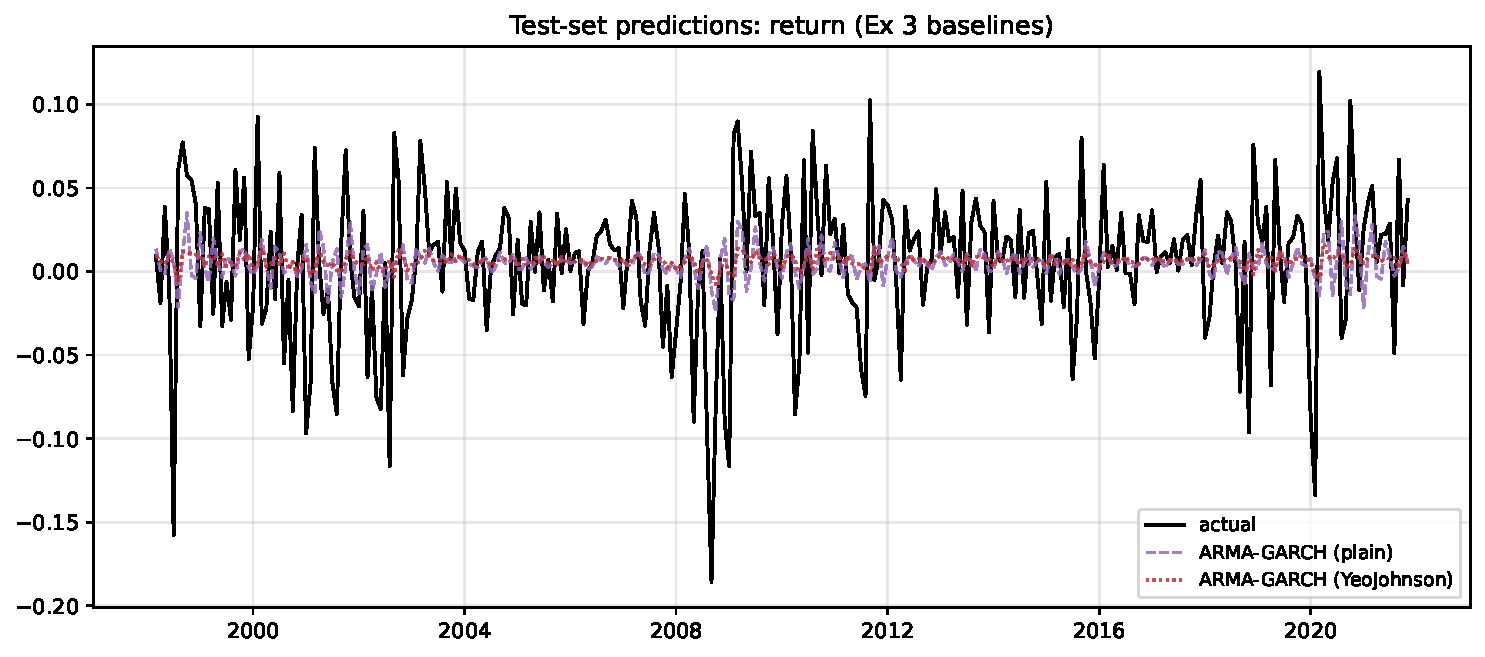
\includegraphics[width=0.95\linewidth]{output/ex3/07_ex3_fig_return.pdf}
\caption{Test-set return predictions. Both ARMA-GARCH variants flatline near zero with small autoregressive ripples (the plain ARMA(2,2) shows slightly more variation than the Yeo-Johnson MA(1)). Compare with Figure~\ref{fig:ex2_return}.}
\label{fig:ex3_return}
\end{figure}

\begin{figure}[H]
\centering
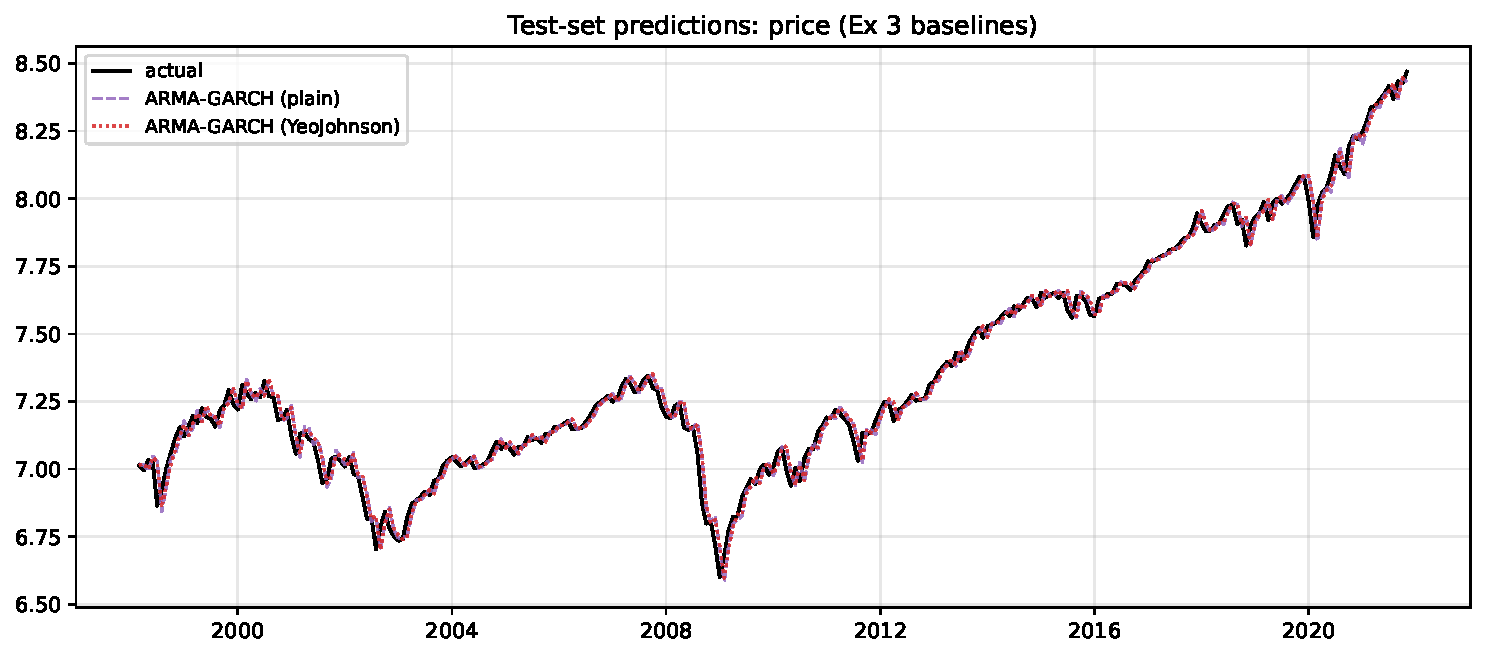
\includegraphics[width=0.95\linewidth]{output/ex3/09_ex3_fig_price.pdf}
\caption{Test-set log-price predictions. Both ARMA-GARCH variants are visually indistinguishable from the actual series, since the predicted log price equals the realised lagged log price plus a small predicted return.}
\label{fig:ex3_price}
\end{figure}

\begin{figure}[H]
\centering
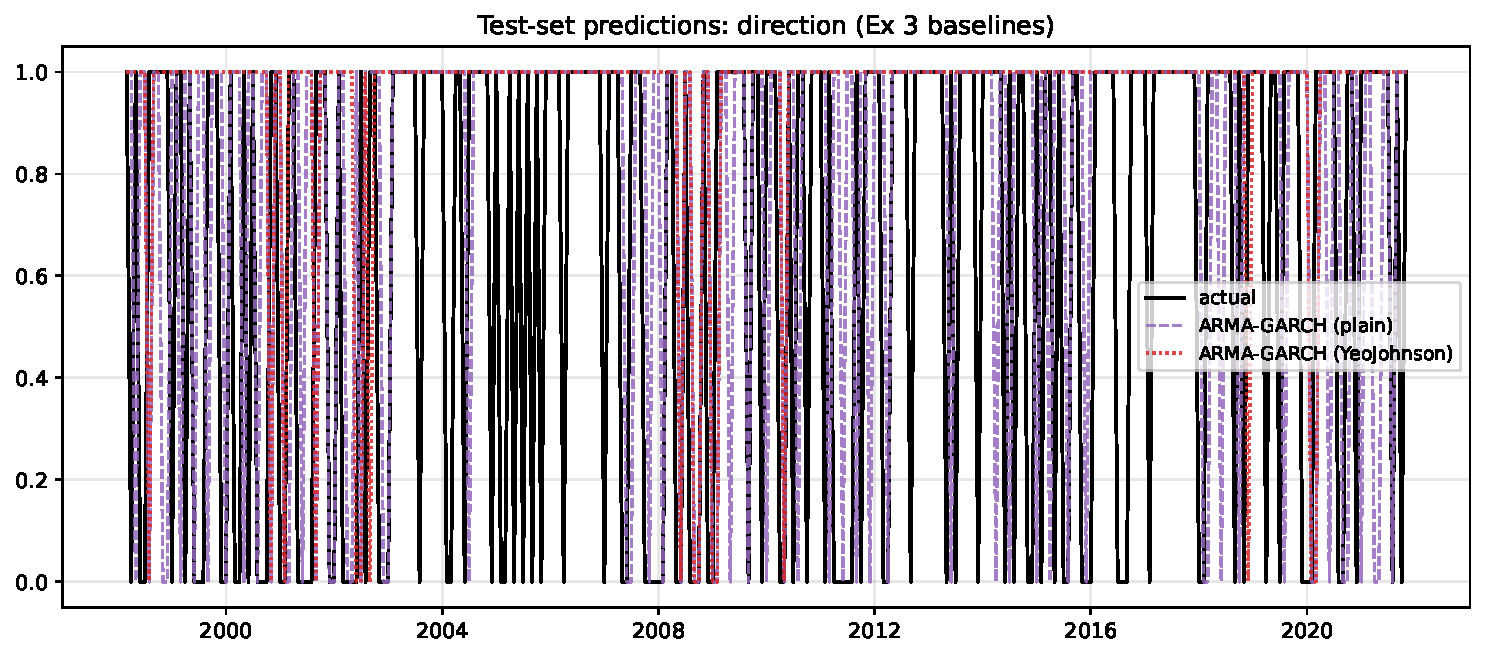
\includegraphics[width=0.95\linewidth]{output/ex3/11_ex3_fig_direction.pdf}
\caption{Test-set direction predictions. Both ARMA-GARCH variants make non-trivial 0/1 calls and produce positive Matthews correlations, while the Exercise 2 GP and BaselineMajority collapse to the majority class and the Exercise 2 NN and LSTM produce non-trivial calls with negative MCC.}
\label{fig:ex3_direction}
\end{figure}

On the return target, the ARMA-GARCH (Yeo-Johnson) variant is the best of the six (NRMSE \exThreeYJReturnNRMSE, marginally below the BaselineMean of \exTwoReturnBaselineMeanNRMSE and the GP of \exTwoReturnGPNRMSE). The plain ARMA-GARCH is essentially tied with the LSTM (\exThreePlainReturnNRMSE against \exTwoReturnLSTMNRMSE), and both ARMA-GARCH variants beat the multilayer perceptron (NRMSE \exTwoReturnNNNRMSE). On the price target both ARMA-GARCH variants beat every Exercise 2 model. The Exercise 2 GP is already 4 times better than the NN and 16 times better than the LSTM in RMSE terms. The simpler ARMA-GARCH baseline still outperforms it by a factor of roughly 1.8 in RMSE. The ARMA-GARCH price forecast is mechanically the realised lagged log price plus a small predicted log return, i.e.\ the optimal random-walk-with-drift forecast for an integrated series. The GP's smooth posterior introduces small additive distortions that the rigid AR-plus-drift structure avoids. The direction target sustains the contrast in favour of ARMA-GARCH. The Exercise 2 GP and BaselineMajority both collapse to ``always up'' with MCC exactly zero. The Exercise 2 NN and LSTM produce non-trivial predictions with negative MCC. Both ARMA-GARCH variants produce small positive MCCs (\exThreePlainDirectionMCC for plain and \exThreeYJDirectionMCC for Yeo-Johnson). The Yeo-Johnson ARMA-GARCH exactly matches the majority-baseline accuracy (\exThreeYJDirectionAccuracy) while flipping a non-zero number of class assignments, the diagnostic for a useful classifier.

The Yeo-Johnson normalisation has a small and consistent positive effect across all three targets. Pulling the marginal distribution closer to Gaussian helps the maximum-likelihood ARMA estimator settle on a more parsimonious model (MA(1) against ARMA(2,2)) and produces marginally better forecasts in every metric. The simpler model also exposes less spurious autocorrelation in small samples, which matters most for the direction target where the gap between predictability and noise is narrowest. Box-Cox would be the natural alternative for strictly positive series such as svar or the price level itself. It is unavailable on the return series because returns are real-valued and frequently negative.

The conclusion of this comparison is that the assignment's framing of ARMA-GARCH as a ``baseline'' understates its strength. On this dataset and this test period the ARMA-GARCH baseline wins on every target where there is anything to win at all, and ties on the one target (return) where nothing wins. The deep models (NN, LSTM and GP) bring no extra predictive value at monthly frequency on the Goyal-Welch indicator set and at least one of them (LSTM on price) is worse than the simplest possible random-walk forecast. This is the standard out-of-sample equity-premium-puzzle picture: classical time-series models, properly fit, are very hard to beat when the underlying signal is weak.

% =============================================================================
% Exercise 4
% =============================================================================
\probsection{4}{Lessons Summary}

Lecture~1 introduces the financial-markets vocabulary that the rest of the course relies on. Securities are classified as debt (bonds), equity (stocks) and derivatives (options, futures and forwards), and we distinguish risky instruments (stocks and options) from risk-free ones (government bonds). We learn the difference between payoff (the value of a security at maturity) and profit (the risk-adjusted payoff that discounts the initial investment). Bond payoffs are computed by compounding interest, with the continuously compounded form $P_{\Delta t} = P_0 e^{r \Delta t}$ as the natural limit and the most convenient algebraically. The lecture also covers market indices, contrasting price-weighted against capitalisation-weighted via the Value-Line and IBEX-style formulas. The conventional OHLC stock-quote table is introduced too: Adjusted Close is the right column to use for return computations because it accounts for splits and dividends.

Lecture~2 turns to the descriptive statistics of financial time series. A first thread is the case for log returns over simple returns: log returns aggregate additively over multiple periods, $r_t[k] = r_t + r_{t-1} + \dots + r_{t-k+1}$, which makes them tractable for statistical models that assume Gaussianity, while simple returns aggregate multiplicatively. The second thread concerns the empirical distribution of returns. Monthly equity returns are approximately bell-shaped, with skewness near zero and a small mean. Shapiro-Wilk, Jarque-Bera and D'Agostino skewness tests typically reject normality at daily and weekly frequencies because of fat tails and excess kurtosis. That motivates the family of invertible normalising transformations (Box-Cox, Yeo-Johnson, logit, hyperbolic-sine and rank-based) bundled in R's \code{bestNormalize} package and used in our Exercise~3. The lecture closes on volatility, defined as the conditional standard deviation of returns and estimated from data using historical (close-to-close), range-based (Parkinson, Garman-Klass) or exponentially weighted moving average (EWMA, RiskMetrics convention $\lambda = \exOneEwmaLambda$) methods. Annualisation proceeds throughout by multiplying by $\sqrt{h}$ where $h$ is the number of periods per year.

Lecture~3 covers parametric and semi-parametric time-series models. It opens with the general modelling paradigm: a series decomposes additively as $X_t = D_t + Y_t$, where $D_t = m_t + s_t$ is a deterministic trend-and-seasonality component (estimated and subtracted by classical Box-Jenkins methods), and $Y_t$ is the stationary stochastic component, modelled as $Y_t = \mathbb{E}[Y_t | \mathcal{F}_{t-1}] + a_t$, i.e.\ a conditional-mean term plus an innovation. From this scaffold the lecture builds outwards into the linear ARMA(p,q) and ARIMA(p,d,q) family. When the series is stationary we fit ARMA directly. When a Dickey-Fuller test rejects stationarity we difference $d$ times and fit ARMA on the differenced series. The nonlinear leg of the discussion is the ARCH/GARCH family for the conditional variance. ARCH$(p)$ makes $\sigma_t^2$ a linear function of past squared innovations and GARCH$(p,q)$ extends this with lagged variances, $\sigma_t^2 = \omega + \sum_{i=1}^p \alpha_i a_{t-i}^2 + \sum_{j=1}^q \beta_j \sigma_{t-j}^2$, with persistence $\sum (\alpha_i + \beta_j) < 1$ required for stationarity. In Exercise~3 we measured persistence of $\exThreePlainPersistence$ for the plain ARMA-GARCH on monthly S\&P 500 returns, the standard near-unit value for equity volatility. The lecture closes by introducing neural networks (feedforward, single-hidden and deep), backpropagation by gradient descent and the universal approximation theorem, with the NRMSE framed as the preferred forecast metric and the 75/25 chronological split as the standard out-of-sample protocol.

Lecture~4 is about model adequacy via causality and bootstrap. It starts with the formal definition of Granger causality: $X$ Granger-causes $Y$ when $Y$ is better predicted using the histories of both $X$ and $Y$ than using the history of $Y$ alone. The test is an $F$-test comparing the residual sums of squares of the unrestricted ($M_f$) and restricted ($M_r$) regressions, with significance at the 5\% level as the conventional cutoff. The multivariate generalisation follows: VAR with lag selection by AIC, HQ or analogous information criteria (\code{VARselect} in R, \code{statsmodels.VAR.select\_order} in Python), together with the practical advice to discard apparent feedback loops, to repeat the analysis on different sampling periods to detect structural breaks and to remember that Granger's test assumes a linear relationship (extensions to nonlinear and conditional causality exist via kernel and information-theoretic methods). The bootstrap section addresses estimator quality: we sample $m$ datasets with replacement from the empirical CDF $\widehat F_n$, compute the statistic $\hat\theta_n^*$ on each resample and use the resulting distribution as a Monte-Carlo approximation to the unknown sampling distribution. The expected proportion of distinct observations in a bootstrap sample is $1 - 1/e \approx 0.632$, and the procedure fails for non-iid data such as time series, where modifications like the block bootstrap or the stationary bootstrap are required.

Lecture~5 covers machine-learning models: recurrent neural networks, LSTMs and Gaussian processes. The recurrent architecture is the starting point. The hidden state $h_t = \sigma(W_h h_{t-1} + W_x x_t + b)$ propagates information forward in time and is trained by Backpropagation Through Time (BPTT), which unrolls the network across the input sequence and applies the chain rule layer by layer. Vanilla RNNs suffer from vanishing and exploding gradients, which prevents them from capturing dependencies of length much greater than ten. The LSTM addresses the vanishing-gradient problem with a gating mechanism (forget, input and output gates) around an internal cell state $C_t = f_t \odot C_{t-1} + i_t \odot \tilde C_t$. LSTMs are the standard architecture for moderately long time-series dependencies, with GRUs as a simpler variant and Transformers as the modern attention-based alternative for very long sequences. Gaussian-process regression rounds out the lecture: a GP is a distribution over functions parameterised by a mean function (often taken as zero) and a kernel $k(x, x')$, with posterior mean for prediction at a test input $x_*$ given by $\bar f_* = K(x_*, X)[K(X, X) + \sigma_n^2 I]^{-1} y$. The choice of kernel (RBF, Matern, polynomial, rational-quadratic and custom additive) encodes our prior assumptions about smoothness, length-scale and the additive structure of the function. In Exercise~2 the custom non-stationary RBF$+$Linear$+$WhiteNoise kernel was the best price-target predictor among the GP variants, the structure expected when the underlying series is a random walk with drift.

% =============================================================================
% Exercise 5: Author contributions
% =============================================================================
\probsection{5}{Author Contributions}

All authors contributed equally.

\end{document}
